\documentclass[]{aiaa-tc}% insert '[draft]' option to show overfull boxes

% \usepackage[margin=1in]{geometry}
\usepackage[noprefix]{nomencl}
\usepackage[section]{placeins}
\usepackage[colorlinks,bookmarks,bookmarksnumbered,citecolor=red,urlcolor=red]{hyperref}
\usepackage{graphicx}
\usepackage{subfig}
\usepackage{cite}
\usepackage{doi}
% \usepackage[caption=false]{subfig}
% \usepackage{booktabs} % better tables
% \usepackage[noend]{algpseudocode}
\usepackage{algpseudocode}
\usepackage{algorithm}
\usepackage{amsmath}
\usepackage{url}
\usepackage{etoolbox}
\usepackage{color}
\usepackage[capitalize]{cleveref}


\newcommand{\crefrangeconjunction}{--}

\newcommand*\Let[2]{\State #1 $\gets$ #2}

\newtoggle{internal}
\togglefalse{internal}
\newcommand{\internal}[1] {\iftoggle{internal}{{\color{blue}\begin{itemize} #1 \end{itemize} }} }

\makenomenclature

\title{Development and Validation of a New Blade Element Momentum Skewed-Wake Model within AeroDyn}

 \author{
  S. Andrew Ning\thanks{Assistant Professor, Mechanical Engineering Department, AIAA Member}\\
  {\normalsize\itshape
   \hspace*{1in}Brigham Young University, Provo, UT\hspace*{1in}}\\
  \and
  Greg Hayman\thanks{Software Engineer, National Wind Technology Center}
  ,\ Rick Damiani\thanks{Senior Engineer, National Wind Technology Center, AIAA Member}
  ,\ and Jason Jonkman\thanksibid{3}\\
  {\normalsize\itshape
   National Renewable Energy Laboratory, Golden, CO}
 }



\begin{document}

\maketitle


\begin{abstract}
Blade element momentum methods, though conceptually simple, are highly useful for analyzing wind turbines and are widely used in many applications including initial aerodynamic analysis, conceptual design, loads and stability analysis, and controls design.  A new version of AeroDyn is being developed to take advantage of new robust solution methodologies, conform to a new modularization framework for NREL's FAST, utilize advanced skewed-wake analysis methods, fix limitations with previous implementations, and to enable modeling of highly flexible and nonstraight blades.  This paper reviews blade element momentum theory and several of the options available for analyzing skewed-inflow.  AeroDyn implementation details are described for the benefit of users and developers.  These new options are compared to solutions from the previous version of AeroDyn and to experimental data.  Finally, recommendations are given on how one might select from the various available solution approaches.
\end{abstract}

\printnomenclature[1cm]
\nomenclature{$a$}{axial induction factor [state]}
\nomenclature{$a^\prime$}{tangential induction factor [state]}
\nomenclature{$\phi$}{local inflow angle [state, output]}
\nomenclature{$W$}{inflow velocity [output]}
\nomenclature{$V$}{velocity}
\nomenclature{$\alpha$}{angle of attack}
\nomenclature{$\theta$}{twist angle (geometric + structural) [input]}
\nomenclature{$\theta_p$}{pitch angle [input]}
\nomenclature{$c$}{chord [parameter]}
\nomenclature{$\rho$}{fluid density [parameter]}
\nomenclature{$\mu$}{dynamic viscosity [parameter]}
\nomenclature{$c_l$}{lift coefficient }
\nomenclature{$c_d$}{drag coefficient}
\nomenclature{$\sigma^\prime$}{local solidity ($B c /(2\pi r)$) [parameter]}
\nomenclature{$F$}{hub/tip correction factor}
\nomenclature{$B$}{number of blades [parameter]}
\nomenclature{$r$}{local radial position [input]}
\nomenclature{$R$}{rotor tip radius [input]}
\nomenclature{$R_{hub}$}{rotor hub radius [parameter]}
\nomenclature{$\gamma$}{yaw angle [input]}
\nomenclature{$\psi$}{azimuth angle [input]}
\nomenclature{$\chi$}{wake skew angle}
\nomenclature{$\Phi$}{precone angle }
\nomenclature{$\Theta$}{tilt angle}
\nomenclature{$C_T$}{local thrust coefficient}
\nomenclature{$C_Q$}{local torque coefficient}
\nomenclature{$\lambda_r$}{local tip-speed ratio}


\section{Introduction}

Blade element momentum (BEM) theory continues to be widely used for wind turbine aerodynamic analysis in applications such as blade design, loads and stability analysis, and controls design.  Recent advances in deriving a robust solution algorithm for BEM theory \cite{Ning2013a}, and establishing a new modularization framework for FAST\cite{Jonkman2013}, have prompted development of a new version of AeroDyn.  One aspect of that development is in the treatment of skewed wakes (for yawed or tilted flows).  The previous version of AeroDyn used only a simple correction method.  Several methodologies for analyzing skewed wakes exist, and it is unclear which formulations are most appropriate and for what conditions.  This paper will not attempt to definitively answer that question, but will describe some of the options that are available in the new version of AeroDyn and show comparisons to experimental measurement campaigns.  The description in this paper also serves as a review of methodologies used to assess skewed wake BEM flows.

Two main approaches are described in this paper, each with several variations.  The first class of methods will be called correction methods.  These methods provide corrections to computed induction factors, power coefficients, or other quantities.  The robust solution method can easily be extended to handle these methods.  The second class of approaches will be called coupled methods.  In these methods the inclusion of skewed-wake effects is integral to the derivation, and the calculation of the axial and tangential induction factors are not separable.  The coupled methods cannot be solved using the new robust solution algorithm, and must use traditional two-dimensional root-finding approaches.

Another important aspect of analyzing a rotor operating in skew is the unsteady aerodynamic behavior of the airfoil sections.  However, this physics is handled in a separate module of AeroDyn and is not discussed here.  

The local airfoil coordinate system used in the derivation of both BEM theories is shown in \cref{fig:csys}.  The z-direction is directed along the blade, the y-direction opposite to the rotational velocity, and the x-direction given by the right-hand rule (nominally in the downwind direction).  This coordinate system is equally valid for downwind turbines, but in both cases assumes that the rotor is rotating clockwise when viewed from upwind.  Note that because the blade may be curved, the coordinate system is local to each section along the blade (\cref{fig:curved}).  Swept blades can also be handled, but it is assumed that sweep is accomplished through shearing, rather than rotation, so that the local airfoils and local coordinate systems are still defined relative to the unswept rotation direction (\cref{fig:swept}).

% \begin{figure}[htbp]
% \begin{center}
% 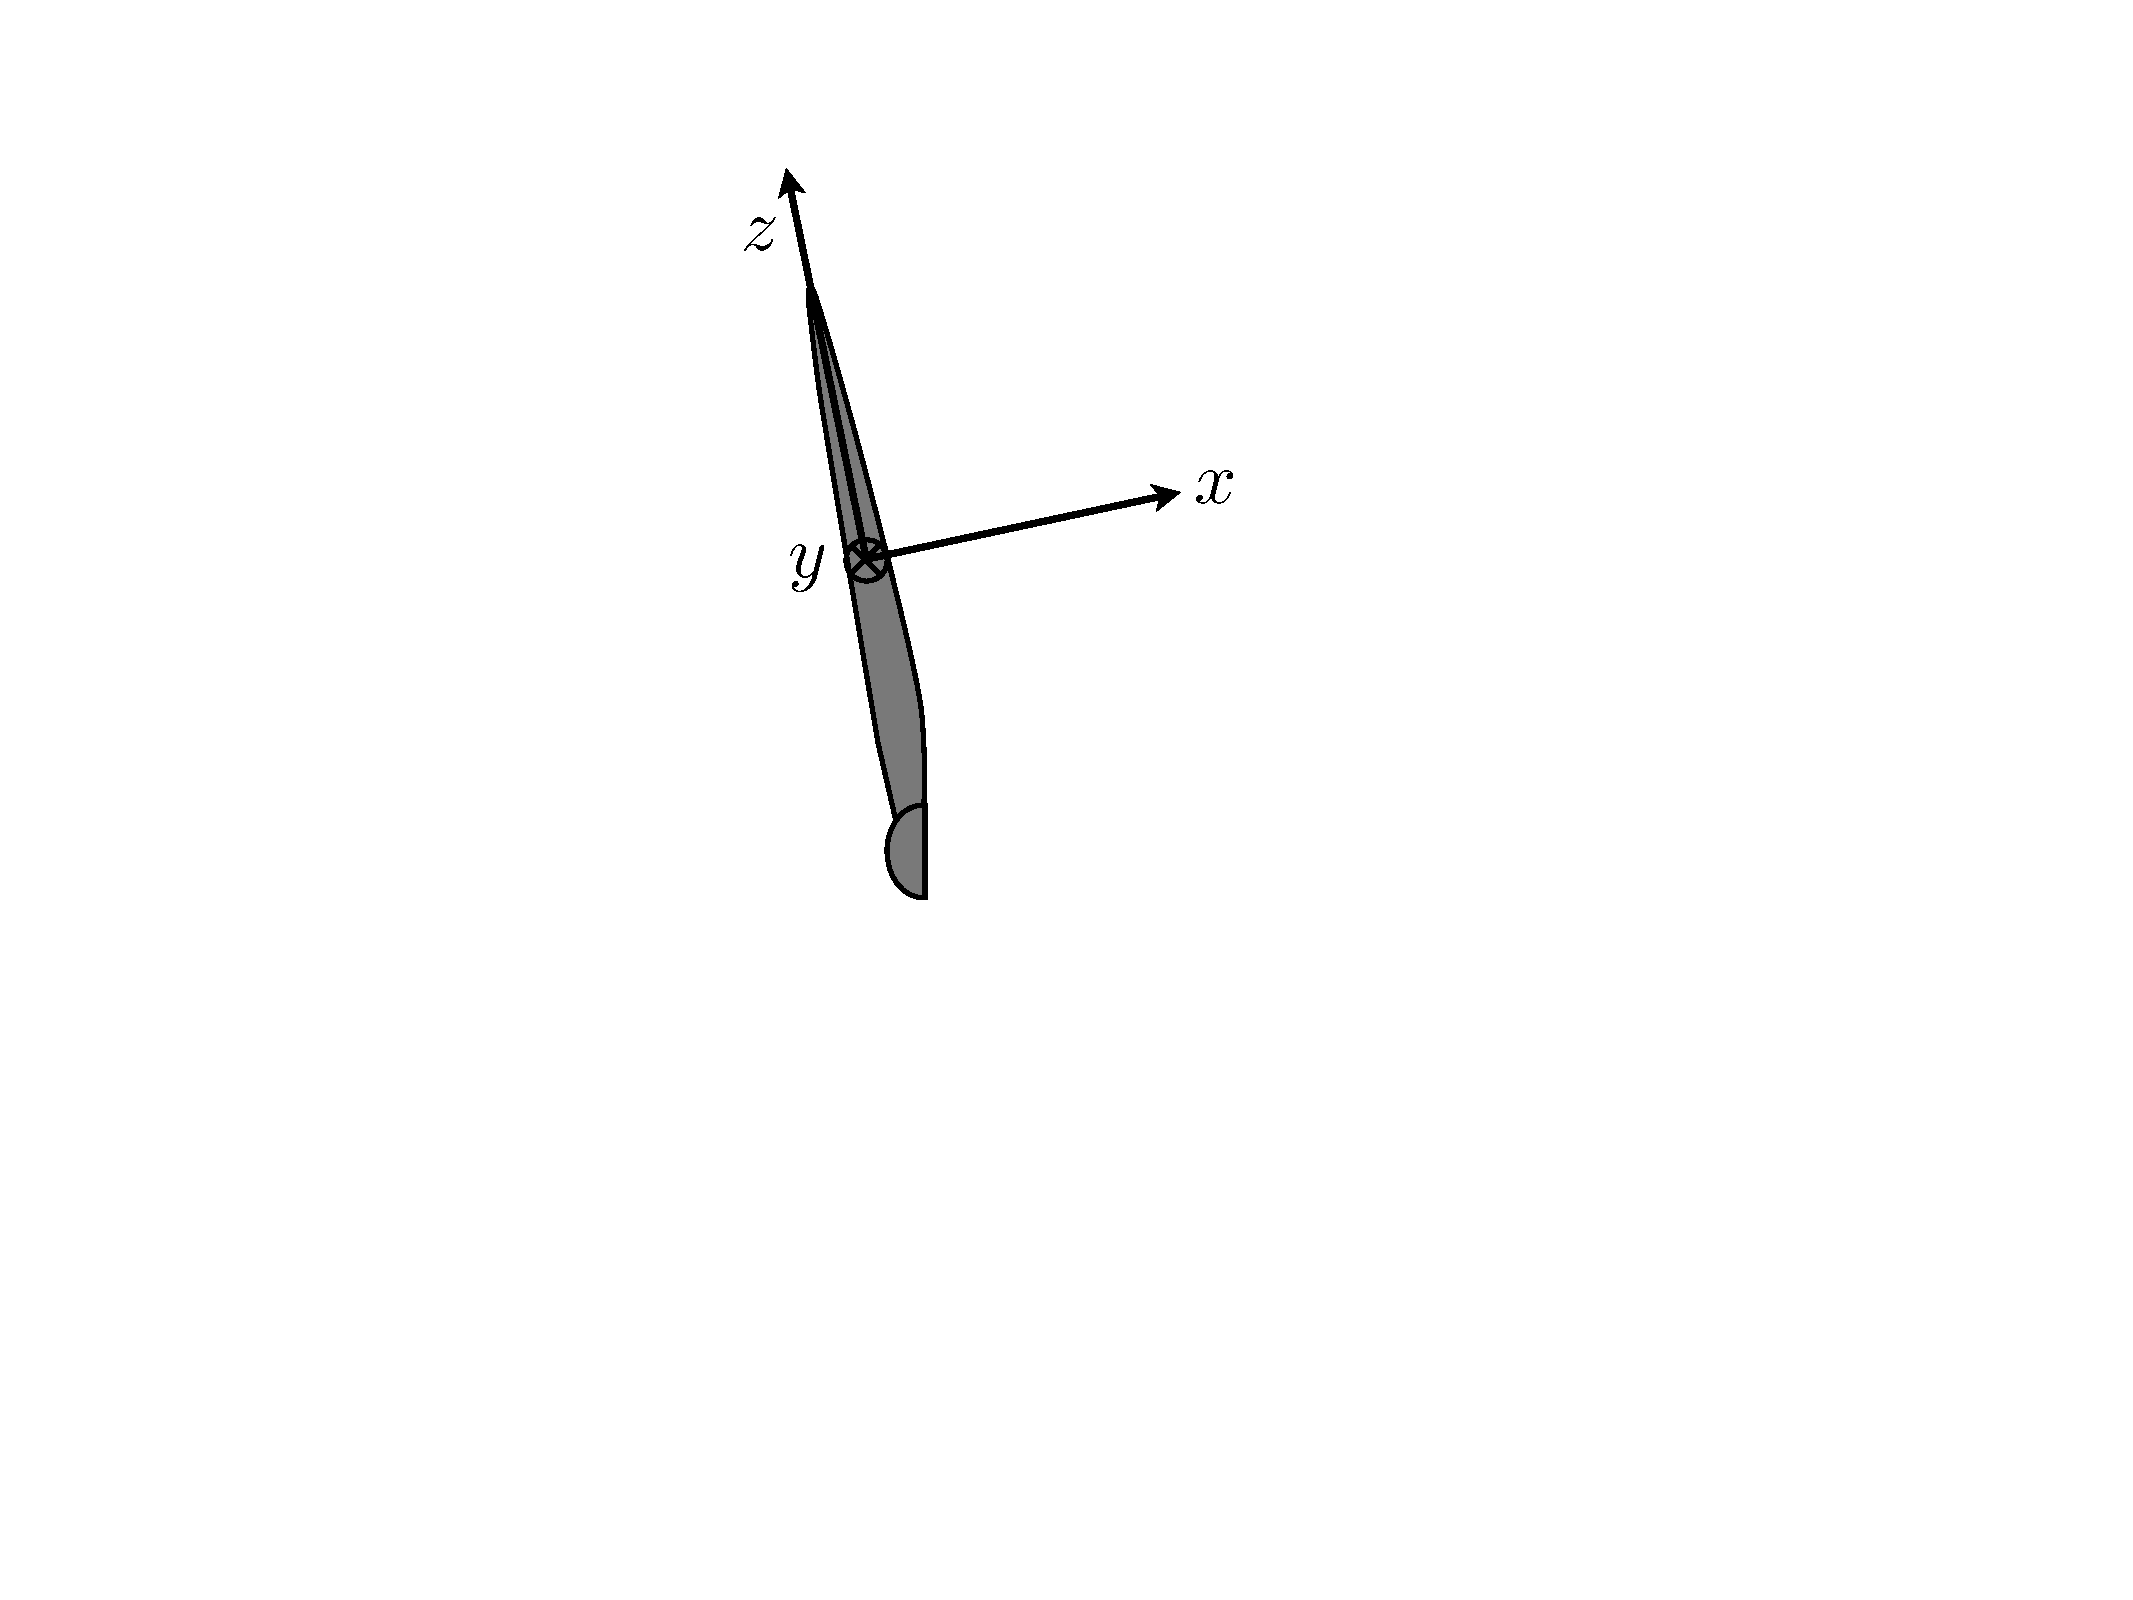
\includegraphics[height=2in]{images/csys}
% \caption{Definition of local airfoil coordinate system.}
% \label{fig:csys}
% \end{center}
% \end{figure}

\begin{figure}[htbp]
\centering
 \subfloat[Side view of curved blade.  Coordinate system is normal to curvature.]{
   \makebox[3.0in][c]{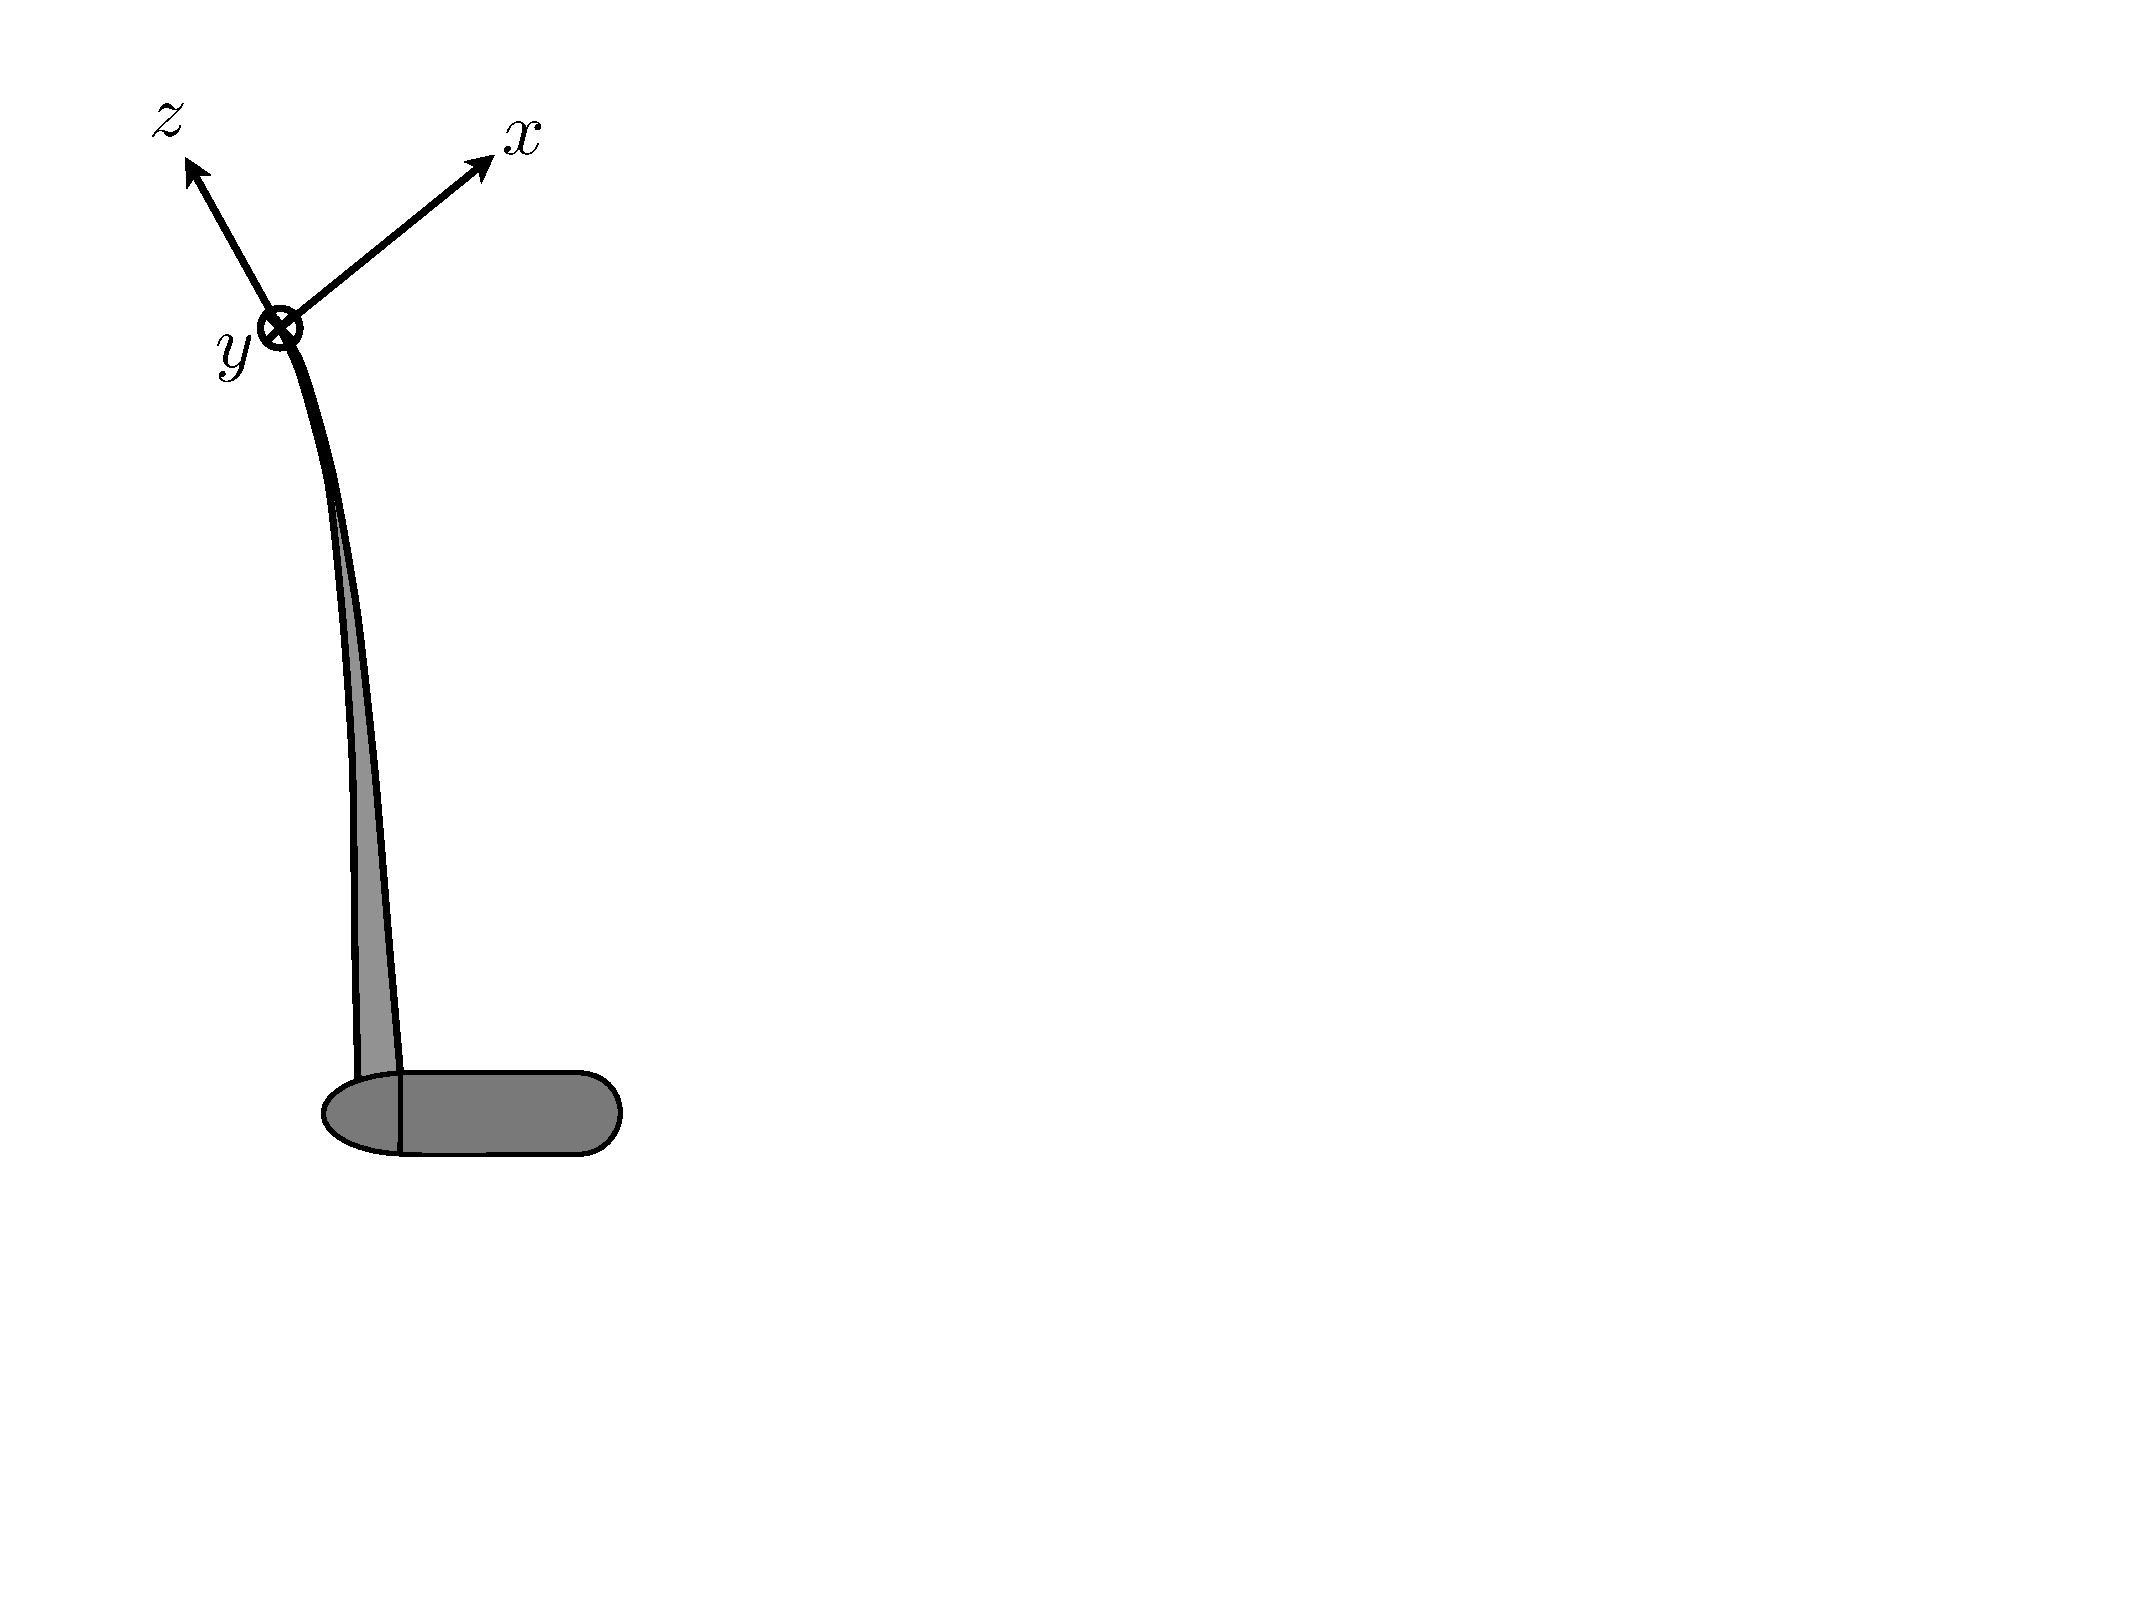
\includegraphics[height=2.5in]{images/curved}}
   \label{fig:curved}
 }
 \qquad
 \subfloat[Front view of swept blade.  Sweep is accomplished through shearing, so coordinate system stays parallel to sweep of blade root.]{
   \makebox[3.0in][c]{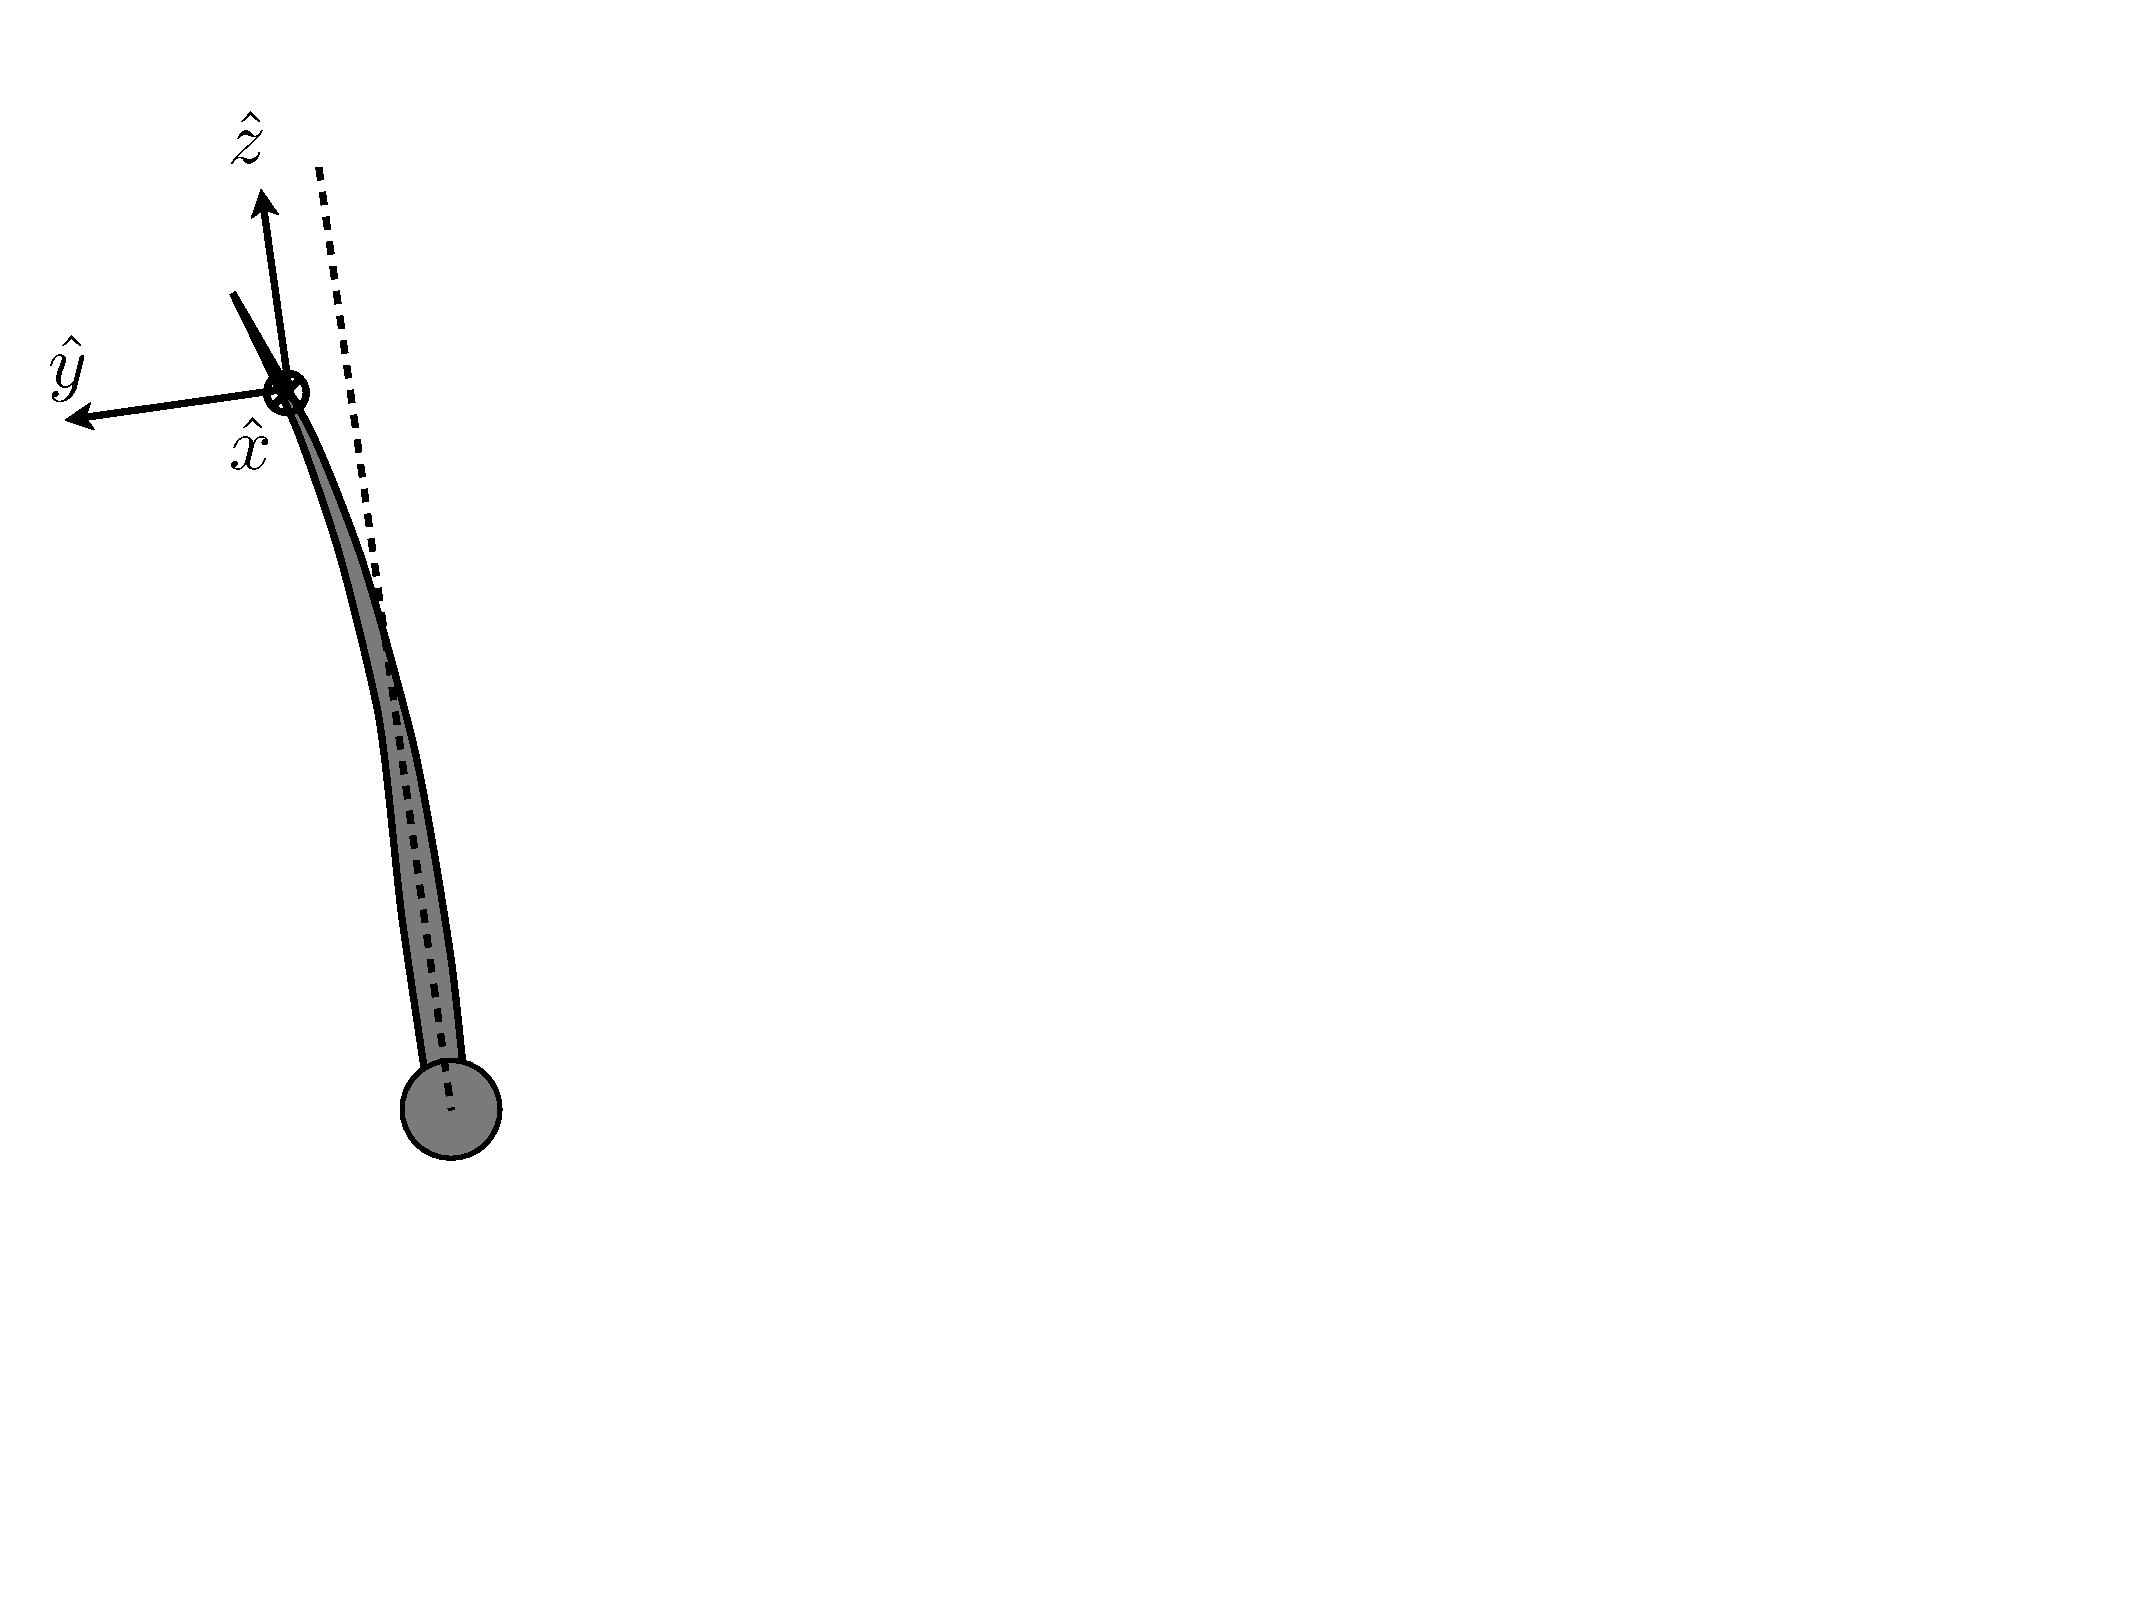
\includegraphics[height=2.5in]{images/swept}}
   \label{fig:swept}
 }
 \caption{Definition of local airfoil coordinate system.}
 \label{fig:csys}
\end{figure}

\section{Classical BEM Theory with a Guaranteed Solution Algorithm}
\label {sec:BEMsolve}
This section reviews the procedure for solving the BEM equations using the guaranteed solution method of Ning \cite{Ning2013a}.  This procedure is based around forming a one-dimensional residual equation as a function of the local inflow angle ($\mathcal{R}(\phi)$).   The definition of the inflow angles and velocity components is seen in \cref{fig:inflow}).  

First, sectional theory is used to compute the force coefficients (\crefrange{eq:alpha}{eq:cy}). In the simplest case, the velocity components are given by $V_x = V_\infty$ and $V_y = \Omega r$, but in the general case the velocity components must also account for shear, turbulence, blade motion, and blade position.  Generally, this is accomplished by using a direction cosine matrix. The Reynolds number can include the induction factors, but that is typically unnecessary because relevant changes in Reynolds number are usually of a much higher order of magnitude than can be caused by changes in induction factor.  The theory permits induction factors to be included in the Reynolds number calculation through an extra iteration loop, but in practice this is very rarely useful \cite{Ning2013a}.  The functions $f_L$ and $f_D$ used in \cref{eq:cl,eq:cd} are often lookup tables from precomputed airfoil data.  In AeroDyn, airfoil force coefficient data is fit with bicubic splines to allow for continuity and differentiability.  In \cref{eq:cx,eq:cy} the drag coefficient is omitted in some implementations, and is optional in AeroDyn.  Note that the positive direction for $c_y$ is opposite the $\hat{y}$ vector by convention.

\begin{figure}[htbp]
\begin{center}
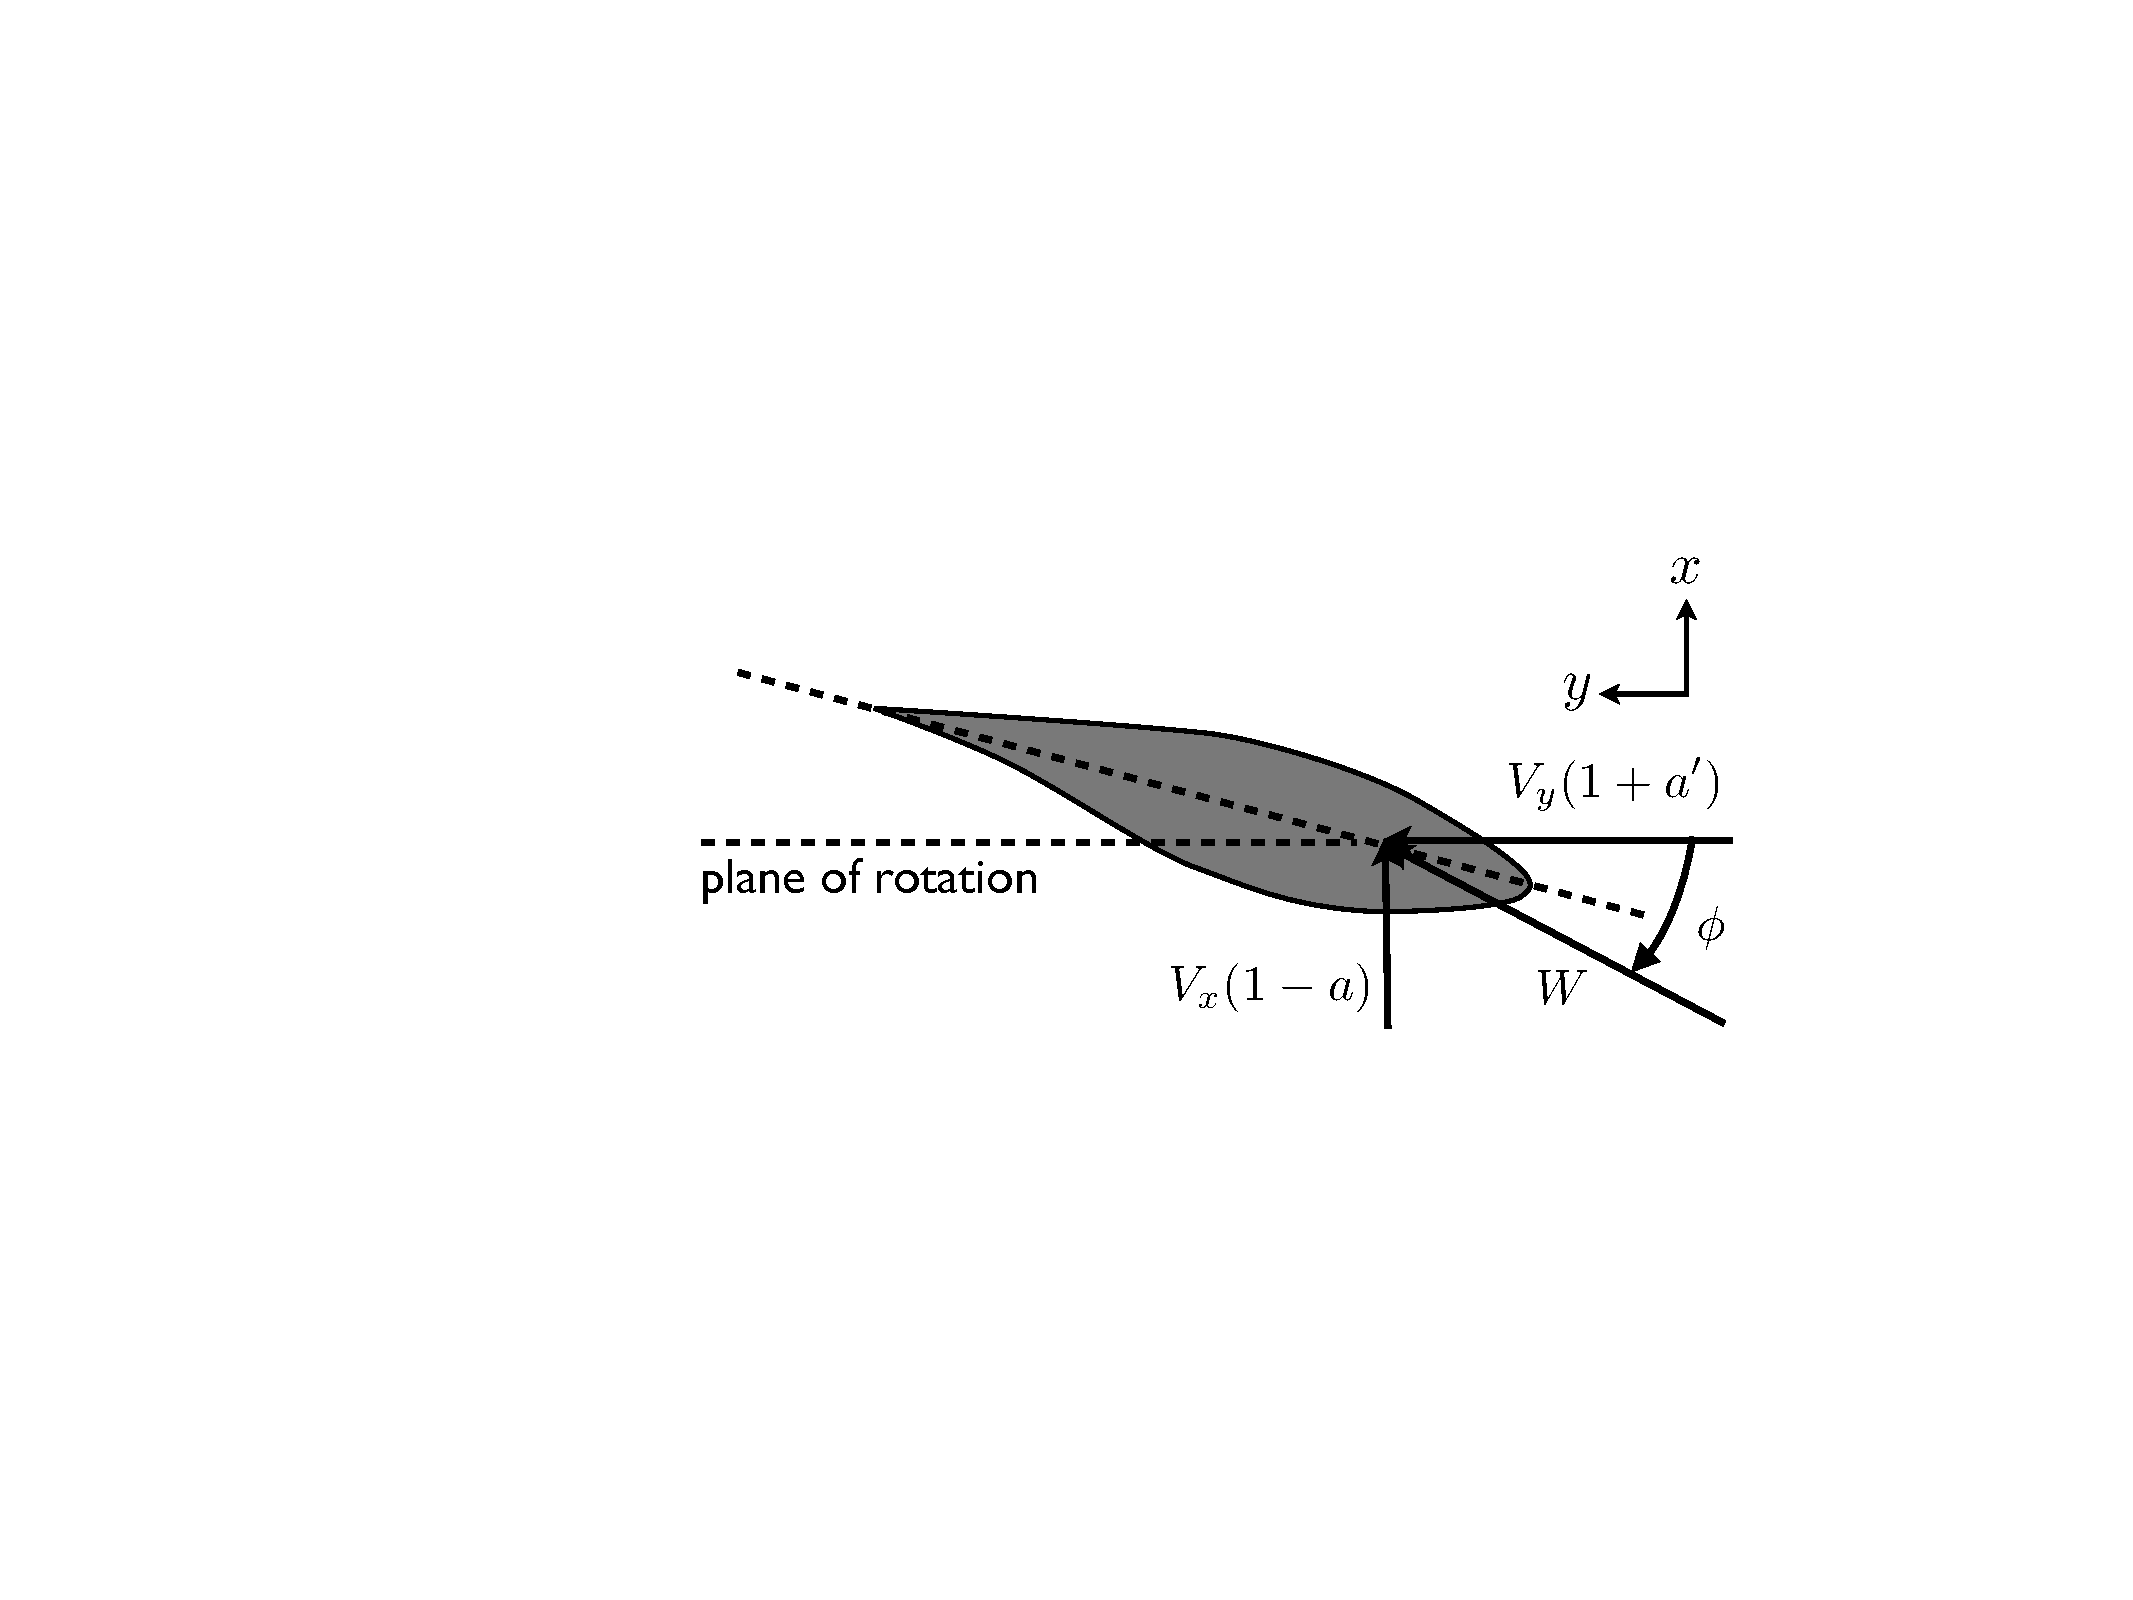
\includegraphics[width=3.5in]{images/inflow}
\caption{Definition of velocity components and inflow parameters for a local rotating blade section.}
\label{fig:inflow}
\end{center}
\end{figure}

\begin{align}
    \alpha &= \phi - (\theta + \theta_p) \label{eq:alpha}\\
    W_\infty &= \sqrt{V_x^2 + V_y^2} \label{eq:W}\\
    Re &= \frac{\rho W_\infty c}{\mu}\label{eq:Re}\\
    c_l &= f_L(\alpha, Re)\label{eq:cl}\\
    c_d &= f_D(\alpha, Re)\label{eq:cd}\\
    c_x &= c_l \cos\phi + c_d \sin\phi \label{eq:cx}\\
    c_y &= c_l \sin\phi - c_d \cos\phi \label{eq:cy}
    % \kappa &= \frac{\sigma^\prime c_n}{4 F(\phi) \sin^2\phi}\\
    % \kappa^\prime &= \frac{\sigma^\prime c_t}{4 F(\phi) \sin\phi\cos\phi}
\end{align}

\internal{
\item Marshall is working on the implementations of $f_L$ and $f_D$. For continuity in derivatives it is essential that this is done using splines.  I use the Fortran package DIERCKX for this.  Specifically the routines \href{http://www.netlib.org/dierckx/regrid.f}{regrid.f} to setup the spline on a uniform grid (for a given airfoil), and \href{http://www.netlib.org/dierckx/bispev.f}{bispev.f} to evaluate the spline.  I force kx, ky to never be larger than 3 (bicubic splines), and I use a smoothing parameter of 0.1 for the lift, and 0.001 for the drag.  This is important to prevent non-physical multiple solutions introduced by poor airfoil data.  The smoothing factor for the lift may be on the large side.  

\item $\theta$ in \cref{eq:alpha} should include both geometric and structural twist.

\item There should be a boolean used to toggle whether or not drag, $c_d$ is included in \cref{eq:cx,eq:cy}.
}


Next, the results of blade element theory are combined with those of momentum theory in order to compute the induction factors.  In the following it is assumed that the empirical region is estimated using Glauert's correction with Buhl's modification\cite{Buhl2005}.  First, two relevant nondimensional parameters are computed
\begin{align}
    \kappa &= \frac{\sigma^\prime c_x}{4 F \sin^2\phi}\\
    \kappa^\prime &= \frac{\sigma^\prime c_y}{4 F \sin\phi\cos\phi}\\
\end{align}
$F$ is a hub/tip loss correction.  AeroDyn uses Prandtl's correction 
\begin{align}
f_{tip} &= \frac{B}{2} \left(\frac{R - r}{r|\sin\phi|} \right)\\
F_{tip} &= \frac{2}{\pi} \arccos(\exp(-f_{tip}))\\
f_{hub} &= \frac{B}{2} \left(\frac{r - R_{hub}}{R_{hub}|\sin\phi|} \right)\\
F_{hub} &= \frac{2}{\pi} \arccos(\exp(-f_{hub}))\\
F &= F_{tip}F_{hub}
\end{align}


Different equations must be used depending on the solution region.  If $\phi > 0$ and $\kappa \le 2/3$ then the solution falls in the momentum region where
\begin{equation}
a = \frac{\kappa}{1 + \kappa}
\end{equation}
Alternatively, if $\phi > 0$ and $\kappa > 2/3$ then the solution falls in the empirical region.
\begin{equation}
a = \frac{\gamma_1 - \sqrt{\gamma_2}}{\gamma_3}
\label{eq:abuhl}
\end{equation}
where
\begin{equation}
\gamma_1 \equiv 2F\kappa - \left(\frac{10}{9} - F\right)\!, \quad \gamma_2 \equiv 2F\kappa - F\left(\frac{4}{3} - F\right)\!,\quad
\gamma_3 \equiv 2F\kappa - \left(\frac{25}{9} - 2F\right)
\label{eq:gamma}
\end{equation}
If the denominator in \cref{eq:abuhl} is exactly zero (i.e., $\gamma_3 = 0$), then the numerator is also exactly zero.  However, the expression can still be evaluated using L'H\^{o}pital's rule and can be shown to be equal to 
\begin{equation}
    % a(\gamma_3 = 0) \rightarrow 1 - \frac{1}{2\srqt{\gamma_2}}
    a \xrightarrow{\gamma_3 \to 0} 1 - \frac{1}{2\sqrt{\gamma_2}}
    \label{eq:aconverge}
\end{equation}
Otherwise if $\phi < 0$ and $\kappa > 1$ then the solution lies in the propeller brake region.
\begin{equation}
    a = \frac{\kappa}{\kappa -1}
\end{equation}
If $\phi < 0$ and $\kappa \le 1$ then this value of $\phi$ cannot possible be a solution to the BEM equations and so we can set $a$ to any value for which the residual is guaranteed to be nonzero.  For this formulation this holds by simply setting $a = 0$.  Finally, the tangential induction factor is given as
\begin{equation}
    a^\prime = \frac{\kappa^\prime}{1 - \kappa^\prime}
\end{equation}
With the induction factors computed, the residual can be calculated as
\begin{equation}
    \mathcal{R}(\phi) = \frac{\sin\phi}{1 - a} - \frac{V_x}{V_y}\frac{\cos\phi}{(1 + a^\prime)}
    \label{eq:residual}
\end{equation}

\internal{
\item In \cref{eq:gamma} numerical errors can exist near $\gamma_3 == 0$, so I use \cref{eq:aconverge} anytime $|\gamma_3| < 1 \times 10^{-6}$.

% \item \Cref{eq:residual} can be simplified algebraically if desired to
% \begin{equation*}
%     \mathcal{R}(\phi) = \frac{\sin\phi}{1 - a} - \frac{V_x}{V_y} \cos\phi (1 - \kappa^\prime)
% \end{equation*}
}


With equations \crefrange{eq:alpha}{eq:residual} comprising the evaluation of the residual $\mathcal{R}(\phi)$, the solution to the residual equation can be found using a root finding method such as Brent's method\cite{Brent1971} as outlined in \cref{alg:brent}.  The solution, $\phi^*$, is plugged back into \crefrange{eq:alpha}{eq:cy} in order to compute the loads.  For the loads calculation the drag coefficient should always be included in \cref{eq:cx,eq:cy}, and the induction factors should be included in evaluating $W$ for use in dimensionalizing the forces.  The normal and tangential loads are
\begin{align}
W &= \sqrt{\left( V_x (1-a)\right)^2 + \left( V_y (1+a^\prime)\right)^2} \label{eq:Wfull}\\
q &= \frac{1}{2}\rho W^2 \label{eq:q}\\
X^\prime &= c_x q c \label{eq:xprime}\\
Y^\prime &= -c_y q c \label{eq:yprime}\\
M_{Z}^\prime &= q c^2 c_m \label{eq:Mzprime}
% M_{Z}^\prime &= q c^2 \left[c_m + \eta(c_x\cos(\theta+\theta_p) + c_y\sin(\theta+\theta_p))\right] \label{eq:Mzprime}
\end{align}
The integration of these loads along the blade for thrust and torque must account for the curvature, coning, and azimuthal orientation of the blades.
% where $\eta$ is the distance from the pitch axis to the airfoil quarter-chord point in units of chord.  The integration of these loads along the blade for thrust and torque must account for the curvature, coning, and azimuthal orientation of the blades.

The BEM equations breakdown if one of the velocity components is exactly zero (i.e., $V_x = 0$ or $V_y = 0$ in \cref{fig:inflow}).  This can occur, for example, in parked conditions or near yaw angles of 90 degrees.  For these cases, AeroDyn sets both induction factors to zero, and computes the loads in the same manner as described in \cref{eq:Wfull,eq:q,eq:xprime,eq:yprime,eq:Mzprime}.


\begin{algorithm}[htbp]
\caption{determine solution $\phi^*$ to BEM equations}
\label{alg:brent}
\begin{algorithmic}

\Function{$zero$}{$f$, $lb$, $ub$}
    \Comment e.g., Brent's method
    \State \Return $x^*$ where $f(x^*) = 0$ for $lb < x < ub$ and $f(lb)f(ub) < 0$
\EndFunction
\\
\Function{bemsolve}{}
    \Let{$\epsilon$}{$1\times 10^{-6}$}
    \Comment{or some other suitably small value}
    \If {$\mathcal{R}(\epsilon)\mathcal{R}(\pi/2) < 0$}
        \Comment{this is almost always true}
        \Let{$\phi^*$}{$zero(\mathcal{R}(\phi), \epsilon, \pi/2)$}
    \ElsIf {$\mathcal{R}(-\pi/4)\mathcal{R}(-\epsilon) < 0$}
        \Comment{propeller brake region}
        \Let{$\phi^*$}{$zero(\mathcal{R}(\phi), -\pi/4, -\epsilon)$}
    \Else
        \Comment{if all else fails, this is guaranteed to contain a solution}
        \Let{$\phi^*$}{$zero(\mathcal{R}(\phi), \pi/2, \pi-\epsilon)$}
    \EndIf
        \Comment{the region $[-\pi/4, -\pi]$ is unnecessary, see \cite{Ning2013a} for details}
    \Let{$a$}{$a(\phi^*)$}
    \Let{$a^\prime$}{$a^\prime(\phi^*)$}

\EndFunction

\end{algorithmic}
\end{algorithm}

\internal{
    \item This implementation is an algebraic constraint state.  For tight coupling, the residual should be computed in CalcConstrStateResidual() and the loads in CalcOutput().  For loose coupling UpdateStates() should just reuse CalcConstrStateResidual() and wrap it with a Brent solver.  For the loose coupling case CalcOutput must be run after UpdateStates has completed.  There one state, $\phi$, per radial station along the blade.  However, each state is independent, and should be solved independently.
    \item The Brent implementation I am using is located here: \url{https://github.com/scipy/scipy/blob/v0.14.0/scipy/optimize/Zeros/brentq.c}
}



\section{Corrections Methods Compatible with Basic BEM Implementations}
\label{sec:simple}
There are multiple approaches to applying skewed-wake corrections to the basic BEM formulation.  From the blade element perspective, the only change needed to account for skew is when computing the in-plane velocity components ($V_x$ and $V_y$ in \cref{eq:W,eq:Wfull}).  As an example, assuming conventional static rotor geometry, the wind components can be computed as
\begin{equation}
\begin{aligned}
V_x &= V_\infty ((\cos \gamma \sin \Theta \cos \psi + \sin \gamma \sin \psi)\sin \Phi + \cos \gamma \cos \Theta \cos \Phi)\\
V_y &= V_\infty (\cos \gamma \sin \Theta\sin \psi - \sin \gamma \cos \psi) + \Omega r \cos\Phi
\label{eq:Vrel}
\end{aligned}
\end{equation}
where the definition of the angles are shown in \cref{fig:angles}.  Positive precone angles ($\Phi$) tilt the blades upwind.  For curved blades and dynamic motion the equations are more complex, but all cases simply involve resolving the velocity components into the local airfoil frame.

\begin{figure}[htbp]
\centering
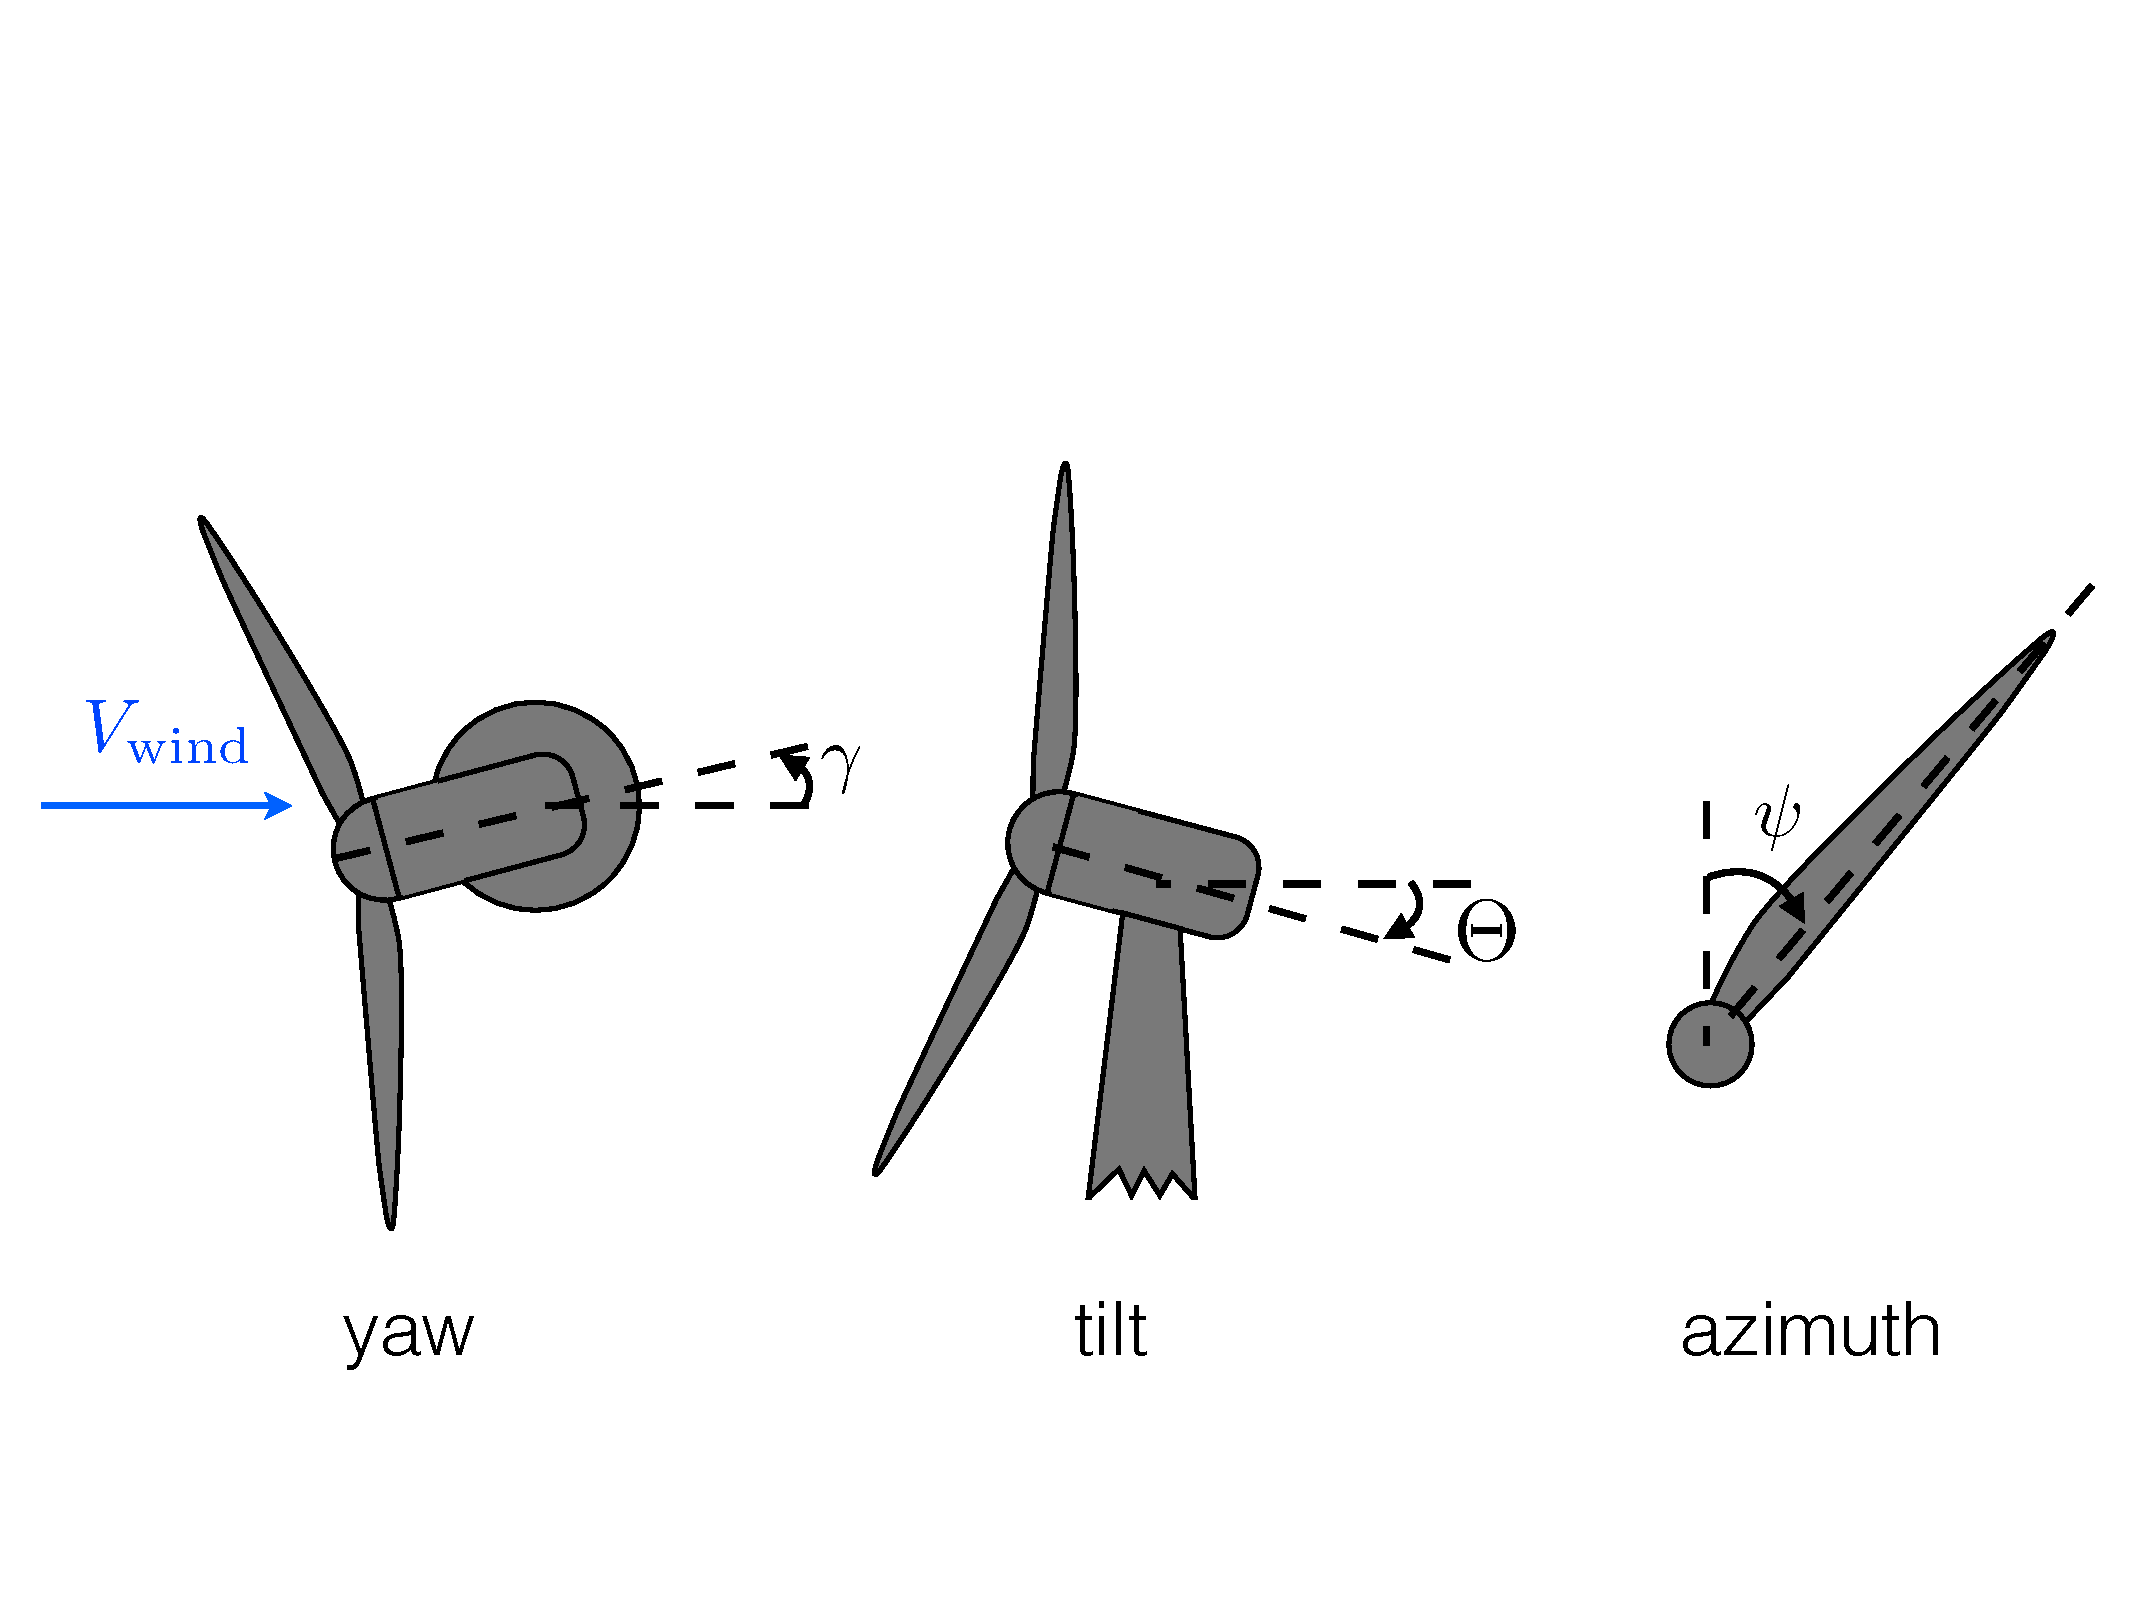
\includegraphics[width=5.5in]{images/angles}
\caption{Definitions for some of the relevant geometric angles.}
\label{fig:angles}
\end{figure}

Often this is the only modification that is applied in basic implementations, but additional corrections can also be made to the momentum side of the formulation.  In developing autogyro theory Glauert proposed a simple nonuniform inflow model in order to better match experimental observations \cite{Glauert1926}.  The induced velocity should decrease toward the leading edge and increase toward the trailing edge.  He proposed a simple linear radial variation with a 1P harmonic variation
\begin{equation}
    a_{yaw} = a \left( 1 + K(\chi) \frac{r}{R}\sin\psi\right)
\end{equation}
where K is some unspecified function, generally expressed in terms of the wake skew angle.  The Pitt and Peters model (static, thrust effect only) was shown to agree well with experimental data as compared to several other simple inflow models \cite{Chen:1989}.  Using the Pitt and Peters model leads to a formulation
\begin{equation}
    a_{yaw} = a \left[ 1 + \frac{15 \pi}{64}\tan\frac{\chi}{2}\frac{r}{R}\sin\psi\right]
    \label{eq:pitt}
\end{equation}
The wake skew angle can be estimated approximately using the relationship from Burton\cite{Burton2011}
\begin{equation}
    \chi = (0.6 a + 1) \gamma
\end{equation}
This equation was written in terms of the yaw angle for simplicity, but more generally in the case of yaw and tilt, $\gamma$ should be replaced with the angle between the wind vector and a vector normal to the rotor plane.

The coefficient used in \cref{eq:pitt} differs from that used in the previous version of AeroDyn.  This implementation uses $15 \pi/64$ as opposed to the factor $15 \pi/32$ that was used previously.  Comparison studies by Snel and Schepers \cite{Snel1995} explored several different yaw models and found a Pitt/Peters model with a coefficient of $15 \pi/64$ to fit best.  The same study also uses a  a nonlinear model from Delft University of Technology that uses a curve fitting approach based on a vortex ring model.  They found that this model exaggerated the amplitude of the correction and removed the nonlinear terms, resulting in a model identical to Pitt/Peters but with a coefficient of 1.  Burton \cite{Burton2011} shows a derivation relating the thrust correction to the axial induction factor which results in a denominator of 32, but that result was derived based on the assumption of small axial induction small $a$.  The original Pitt papers \cite{Pitt1981} suggest that a denominator of 64 is appropriate for correcting thrust.  In our comparisons to experimental data we also found that the smaller factor, $15 \pi/64$, resulted in a better fit.  In addition, for coefficients larger than 1, a small minority of cases would cause the induction factor to become larger than 1 creating singularities in the solution space.  Using a coefficient smaller than 1, like $15 \pi/64$, removed those instabilities.


% Glauert's autogyro theory \cite{Glauert1926} predicts a nonuniform induced inflow for yawed rotors of the form
% \begin{equation}
%     a_{yaw} = a \left( 1 + K(\gamma) \frac{r}{R}\sin\psi\right)
% \end{equation}
% where K is some unspecified function of the yaw angle.  Pitt and Peters \cite{Pitt1981} derived a static model for this formulation
% \begin{equation}
%     a_{yaw} = a \left[ 1 + \frac{15 \pi}{64}\tan\frac{\chi}{2}\frac{r}{R}\sin\psi\right]
% \end{equation}
% %TODO: is it 32 or 64 and is it sin or cos of psi
% This is the correction applied in the previous version of AeroDyn.  An alternative correction is provided by AB\cite{Snel1995}
% \begin{equation}
%     a_{yaw} = a \left[ 1 + 0.63\frac{r}{R}\left(1 + 1.56\left(\frac{r}{R}\right)^2\right)(c_1 + c_2\lambda + c_3\lambda^2 + c_4\lambda^3)\chi\sin\psi\right]
% \end{equation}
% where $c_1 = 2.6296\times10^{-3}$, $c_2 = 1.6222\times10^{-3}$, $c_3 = -1.11111\times10^{-5}$, $c_4 = -3.703710\times10^{-6}$, and $\chi$ is in degrees.  The wake skew angle can be estimated approximately using the relationship from Burton\cite{Burton2011}
% \begin{equation}
%     \chi = (0.6 a + 1) \gamma
% \end{equation}

Many other momentum correction methods exist, but for all the solution procedure is exactly the same as the non-yawed case.  The only modification is that $a_{yaw}$ is used in \cref{eq:residual} instead of $a$. 


\section{Coupled Method}
\label{sec:coupled}
The correction methods of \cref{sec:simple} are simplifications in that the inclusion of a skewed wake affects only directly affect the axial component of the velocity.  In reality, the momentum in both the axial and tangential directions are coupled.  A coupled formulation is described by Burton\cite{Burton2011}.  For this formulation, the two BEM equations cannot be reduced to one in the same way they are in the previous section because the axial and tangential induction factors are coupled.  The coupling leads to a complicated equation for the magnitude of the inflow velocity
\begin{align}
    \left(\frac{W}{V_\infty}\right)^2 &= \left[\frac{V_x}{V_\infty} \left( \cos\gamma - a\right) + \frac{V_y}{V_\infty} a^\prime \sin\chi\cos\psi(1 + \sin\chi\sin\psi)\right]^2 \\
    &+ 
    \left[\frac{V_y}{V_\infty} \left( 1 + a^\prime\cos\chi(1 + \sin\chi\sin\psi)\right) + \frac{V_x}{V_\infty} \cos\psi (a \tan\frac{\chi}{2} - \sin\gamma) \right]^2
\end{align}

With the velocity the blade element expression for thrust coefficient is the familiar one, while the angular momentum is complicated slightly by yaw
\begin{align}
    {C_T}_{element}  &= \left(\frac{W}{V_\infty}\right)^2\sigma^\prime c_x\\
    {C_Q}_{element} &= \left(\frac{W}{V_\infty}\right)^2\sigma^\prime (c_y \cos\chi - c_x\sin\chi\cos\psi)
\end{align}
For momentum theory there are various options.  Glauert's theory leads to 
\begin{equation}
    {C_T}_{momentum} = 4 a F \sqrt{1 - a (2 \cos\gamma - a)}
\end{equation}
while vortex theory leads to
\begin{equation}
    {C_T}_{momentum} = 4 a F \left( \cos\gamma + \tan\frac{\chi}{2}\sin\gamma - a \sec^2\frac{\chi}{2}\right)
\end{equation}
The angular momentum equation is
\begin{equation}
    {C_Q}_{momentum} = 4 \lambda_r a^\prime F (\cos\gamma - a )(\cos^2\psi + \cos^2\chi \sin^2\psi)
\end{equation}
Equating the force coefficients from linear an angular momentum gives two residual equations
\begin{align}
    \mathcal{R}_1(a, a^\prime) &= {C_T}_{element} - {C_T}_{momentum}\\
    \mathcal{R}_2(a, a^\prime) &= {C_Q}_{element} - {C_Q}_{momentum}
\end{align}

The momentum theory is derived on the basis of the entire rotor disc.  However, like classical BEM theory, it is generally applied an annual ring.  In that case, the forces and moments should be integrated around the azimuth.  In the previous equations the azimuthal integration was ignored for simplicity and the equations were applied directly at a given azimuth.  An azimuthal average value of the thrust and torque coefficient for the blade element portion is given by
\begin{align}
    {C_T}_{element} &= \frac{\sigma^\prime}{2\pi}\int_0^{2\pi}\left(\frac{W}{V_\infty}\right)^2 c_x d\psi\\
    {C_Q}_{element} &= \frac{\sigma^\prime}{2\pi}\int_0^{2\pi} \left(\frac{W}{V_\infty}\right)^2(c_y \cos\chi - c_x\sin\chi\cos\psi) d\psi
\end{align}
For momentum theory, the thrust component has no azimuthal variation and so its equation is unchanged, while the torque coefficient can be integrated analytically as
\begin{equation}
    {C_Q}_{momentum} = 2 \lambda_r a^\prime F (\cos\gamma - a)(1 + \cos^2\chi)
\end{equation}
Instead of recomputing the force coefficients along the azimuth at each time step, we save the time history of the force coefficients from the past revolution to use in the integration.  Thus, we are using a running azimuthal average, rather than an instantaneous one.

The solution approach must be modified because there are now 2 state variables at each radial section ($a$ and $a^\prime$).  Brent's method can no longer be used, an an n-dimensional root-finding algorithm needs to be used.  AeroDyn first uses Newton's method to solve the residual equations, and in case of failure uses a Levenberg-Marquardt algorithm.  Once the induction factors are found, the distributed loads are computed in the same way (\crefrange{eq:Wfull}{eq:yprime}).

\internal{
    \item I actually have no idea which n-dimensional algorithms will work best for this new approach.  You will have to test various approaches and see.    
}



\section{Implementation and Changes in AeroDyn}


The latest version of AeroDyn (v15) is being overhauled to adhere to the modularization framework \cite{Jonkman2013}.  AeroDyn provides the aerodynamics modeling capabilities for NREL's FAST wind turbine aero-hydro-servo-elastic simulation tool (\cref{fig:FAST1}).  The BEMT sub-module, implements the BEM equations and solution algorithm (\cref{fig:FAST2}).  In this process, the code has been revised and new theoretical approaches have been implemented or are in the process of being integrated within the software. The BEM and Generalized Dynamic Wake (GDW) methods are independent sub-modules of AeroDyn.  As with many other AeroDyn sub-modules, such as Dynamic Stall, they can be enabled through input file settings.  Here we focus on the most relevant differences between AeroDyn v15 and v14 as they relate to the BEMT sub-module, and implementation details pertinent to the topic discussed in this study.

\begin{figure}[htbp]
\centering
 \subfloat[Conceptual diagram of FAST and its modular interface.]{
   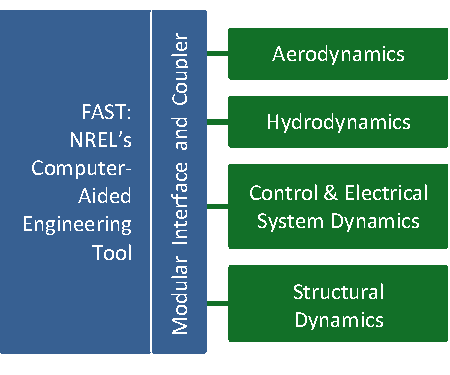
\includegraphics[width=0.45\textwidth]{images/FAST1}
   \label{fig:FAST1}
 }
 \qquad
 \subfloat[The BEMT module is a sub-module within AeroDyn]{
   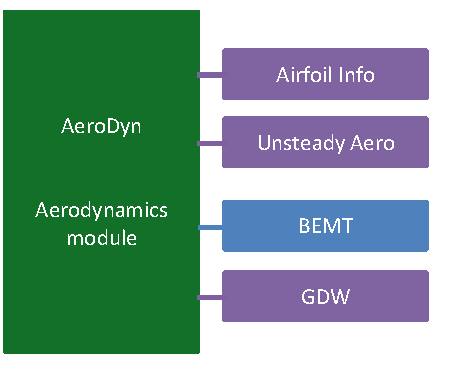
\includegraphics[width=0.45\textwidth]{images/FAST2}
   \label{fig:FAST2}
 }
 \caption{AeroDyn is a module within NREL's FAST, an aero-hydro-servo-elastic simulation tool.  The focus of this study was on AeroDyn's BEMT sub-module.}
 \label{fig:FAST}
\end{figure}
 


\subsection{Implementation in FAST Framework}

Following the requirements of the modularization framework, we establish the inputs, outputs, states, and parameters that allow the BEM equations to be properly coupled to AeroDyn (and in turn FAST).  Within the framework, static quantities are specified during the module's initialization and are stored as parameters.  For the BEMT module these parameters include the rotor geometry, air density, kinematic viscosity, airfoil properties associated with each blade node, and BEMT algorithm options.  These options include selection of the skewed wake correction method, use of drag ($C_d$) when computing $C_x$ and $C_y$, application of the Prandtl hub/tip loss corrections, and the inclusion of the tangential induction factor ($a'$) in the solution.  The algorithm of \cref{sec:simple} includes the ability to iterate on Reynolds number.  However, Aerodyn v15 does not implement this addition iteration loop.

During time-marching, AeroDyn provides BEMT with the required time-dependent inputs relating to the blade node positions and displacements.  These inputs are specified for the entire rotor, for a given blade, or for a specific blade node location.  The rotor-related inputs are, angular velocity ($\Omega$), and yaw angle ($\gamma$).  For each blade, AeroDyn specifies the azimuthal position ($\psi$).   The following inputs are required at each blade node:  the local twist angle ($\theta$), the local inflow velocities ($V_x$ and $V_y$), and the node's radial distance from the center-of-rotation.  The latter accounts for blade deformations.  

The required state variables depends on whether the user selected an uncoupled skewed wake correction from \cref{sec:simple}, or a coupled correction from \cref{sec:coupled}. For the uncoupled corrections, the state variable is the inflow angle ($\phi$), at each blade node.  For coupled skewed wake corrections, the state variables become the axial and tangential induction factors ($a$, $a^\prime$).  

The AeroDyn module uses the BEMT outputs of $W$, $\phi$, $c_x$, and $c_y$ to compute the loads of equations 25-27.

The BEMT sub-module implements the solution algorithms described in \cref{sec:BEMsolve} using three key interface routines of the FAST modularization framework: CalcConstrStateResidual, UpdateStates, and CalcOutput, (\cref{fig:AD_FAST}).

\begin{figure}[htbp]
\centering
 \subfloat[The CalcConstrStateResidual subroutine.]{
   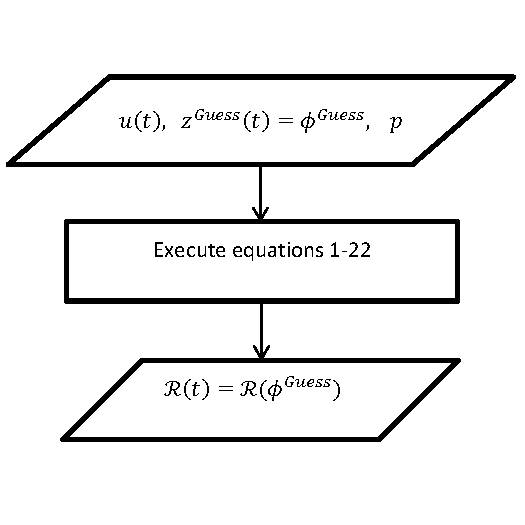
\includegraphics[width=0.45\textwidth]{images/aerodyn_ccsr}
   \label{fig:AD_CCSR}
 }
 \qquad
 \subfloat[The UpdateStates subroutine.]{
   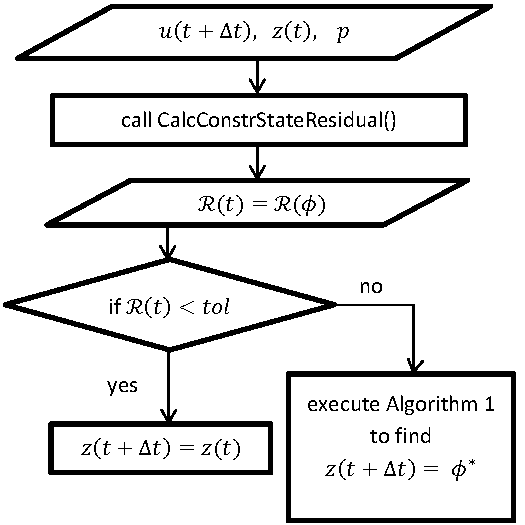
\includegraphics[width=0.45\textwidth]{images/aerodyn_us}
   \label{fig:AD_US}
 }
 \qquad
 \subfloat[The CalcOutput subroutine.]{
   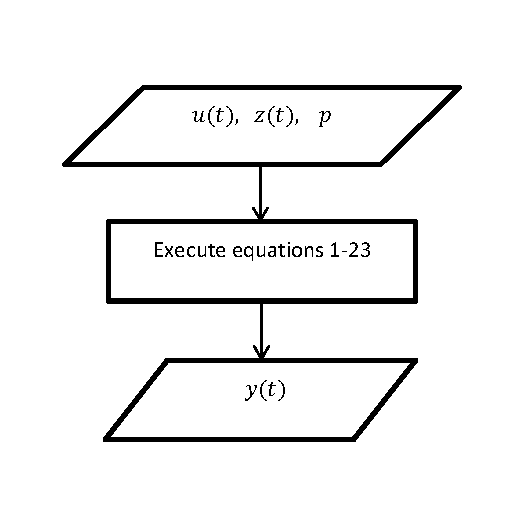
\includegraphics[width=0.45\textwidth]{images/aerodyn_co}
   \label{fig:AD_CO}
 }
 \caption{The uncoupled BEM solution technique as implemented in the BEMT sub-module via the FAST modularization framework.}
 \label{fig:AD_FAST}
\end{figure}


\subsection{Primary Changes in New Version of AeroDyn}
AeroDyn v15 adopts a restructured handling of the airfoil data via the Airfoil Info sub-module. The $C_l$-$C_d$-$C_m$ airfoil coefficient data tables, which are a function of angle of attack, Reynolds number, and possible aerodynamics-control setting (e.g., flap setting), are now interpolated via cubic-splines, whereas previously, a linear interpolation was used. The new scheme is also based on logarithmic values of the Reynolds number for improved accuracy in the interpolation.  A future release of AeroDyn will implement corrections to 2D airfoil data to account for rotational augmentation effects and delayed stall effects.

When calculating the induction factor, Aerodyn release (v14) had a simple iteration loop where the convergence was based on the difference between two successive iteration values of the axial induction factor alone.  The loop also made use of a relaxation factor to assign the new step to the induction factor.  The tangential induction factor was decoupled, and calculated at each iteration based on the axial induction. The body motion contribution to the axial velocity was not corrected for induction, and no elastic-body motion contribution was considered in the calculation of the effective in-plane velocity, (the latter is considered an unintentional bug).  Within the tangential induction calculation, the critical phi values of $0^\circ$ and $90^\circ$ were avoided, limiting the cosine and sine of the inflow angle to 0.01.

AeroDyn v15 adopts a new solution method as described in \cref{sec:simple}, where $a$ and $a^\prime$ are solved simultaneously. Additionally, the body motion is added to the wind in- and out-of-plane components.  This seems more appropriate from a pure aerodynamics stand-point, especially for larger wind turbines where turbulence and structural dynamics time scales may be closer to each other.  

%Since $\phi$ is the primary value returned by the iterator, AeroDyn now sets the axial and tangential induction factors to zero in the cases where $\phi$=$90^\circ$ and $\phi$=$0^\circ$.  TODO: address this

Another important difference between the two versions of AeroDyn is that the skewed wake correction (e.g., Pitt-Peters) is implemented within the iterator in the current release as opposed to a-posteriori in v14. % This is deemed to be more in line with the real physics and has been shown to produce better results (See Section ZZZ and figures YYY) when compared to experimental data.

The AeroDyn v14 loosely implemented the Pitt-Peters method by including a factor dependent on the disk-averaged angle of attack ($\alpha_d$), and a correction factor of $15 \pi / 32$. AeroDyn v15 uses the skew angle ($\chi$) in place of $\alpha_d$, and a correction factor of $15 \pi / 64$.





% \section{Comparison to Previous Version of AeroDyn}
% [This section will compare how this new version compares to AeroDyn v15, including what functionality is new and how the results are different.]

\section{Comparison to Experimental Data}
In this section we make comparison of simulation results to the data from the NREL Unsteady Aerodynamics experiment \cite{Hand:2001}.  Tests were conducted at the NASA 80 x 120 wind tunnel with a 20 kW horizontal-axis wind turbine.  A large variety of tests were conducted, but this paper focuses on comparison with the ``upwind baseline'' test series. All input values were either taken directly from the report or from the experimental data files. [TODO: Jason can you describe the airfoils used, and the selection of stations]  A small shear exponent of 0.05 was used, as was consistent with the experimental data.  At a given azimuth angle, outputs (and some measured inputs) shows small variations during the 30-second measurements, and so average values were used for each azimuthal location.  In all of the figures of this section closed circles are used to signify experimental data, while continuous lines represent simulation results.  Distributed loads in the x-direction are referred to as flapwise, while loads in the y-direction are referred to as lead-lag.  

\subsection{Correction Methods}

The first comparison is done at zero yaw, and so is a comparison between basic BEM theory and the experimental data.  Figure \ref{fig:Uinf} compares the distributed loads along the blade at three different wind speeds.  Each case is done at $0^\circ$ yaw, and $90^\circ$ azimuth.  Because the shear is so small and the yaw angle is zero, the computational and simulation results differ only slightly as a function of azimuth angle.  The BEM model generally shows good agreement to the experimental data except at the inboard sections for high wind speeds.  The discrepancy is caused because those sections are operating beyond the airfoil's stall angle and we do not include a dynamic stall model in these results. The purpose of this study is to isolate the effect of the yaw models and so we specifically restrict our focus to low wind speeds where different stall models (or lack thereof) would confound the results.  At the lower wind speeds, and outboard at 10 m/s, we note that the lead-lag loads are predicted quite well.  This is important because those are the loads that primarily affect power prediction.  The flapwise loads primary change the thrust load and are well predicted inboard but appear to be overpredicted toward the blade tips.  All of the following figures are done at a constant wind speed of $V_\infty = 7$ m/s.


\begin{figure}[htbp]
\centering
 \subfloat[5 m/s]{
   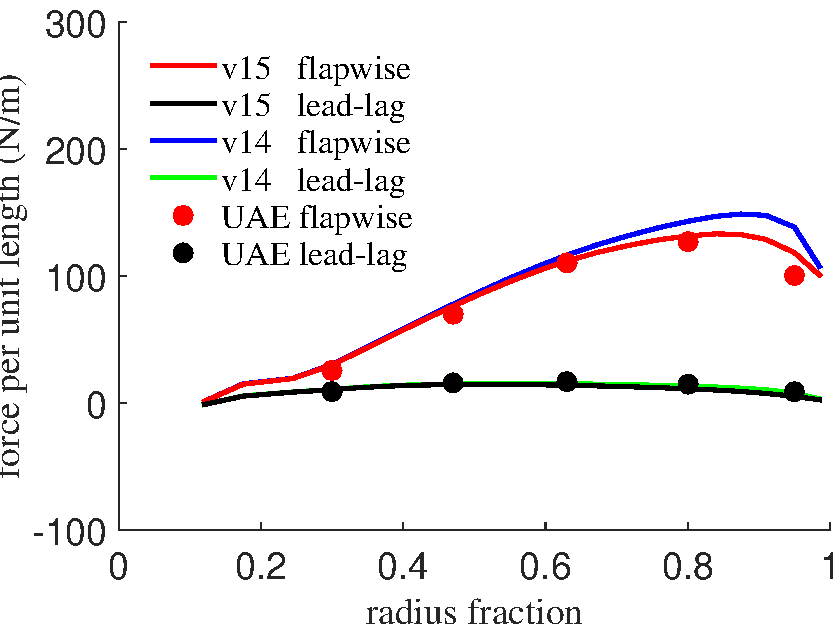
\includegraphics[width=0.3\textwidth]{images/Uinf_5}
   \label{fig:Uinf_5}
 }
 \quad
 \subfloat[7 m/s]{
   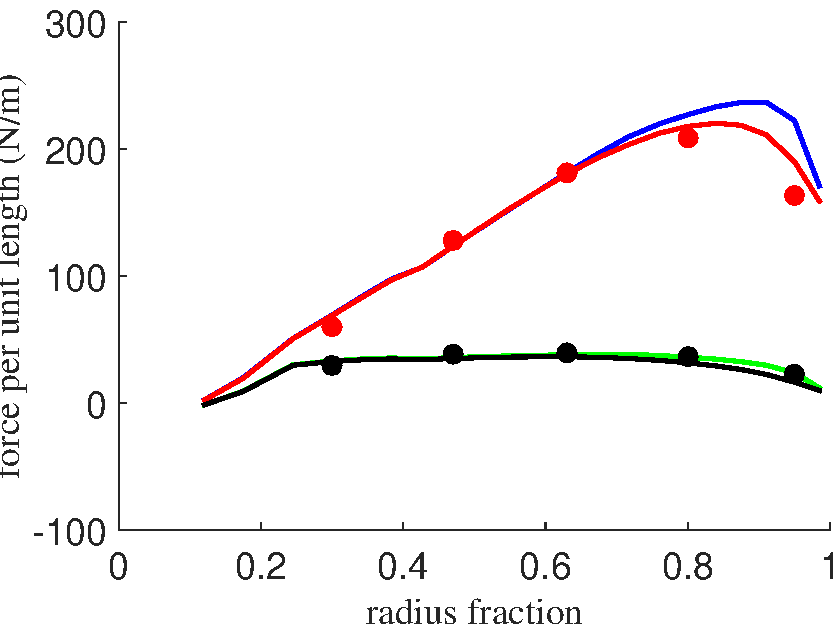
\includegraphics[width=0.3\textwidth]{images/Uinf_7}
   \label{fig:Uinf_7}
 }
 \quad
 \subfloat[10 m/s]{
   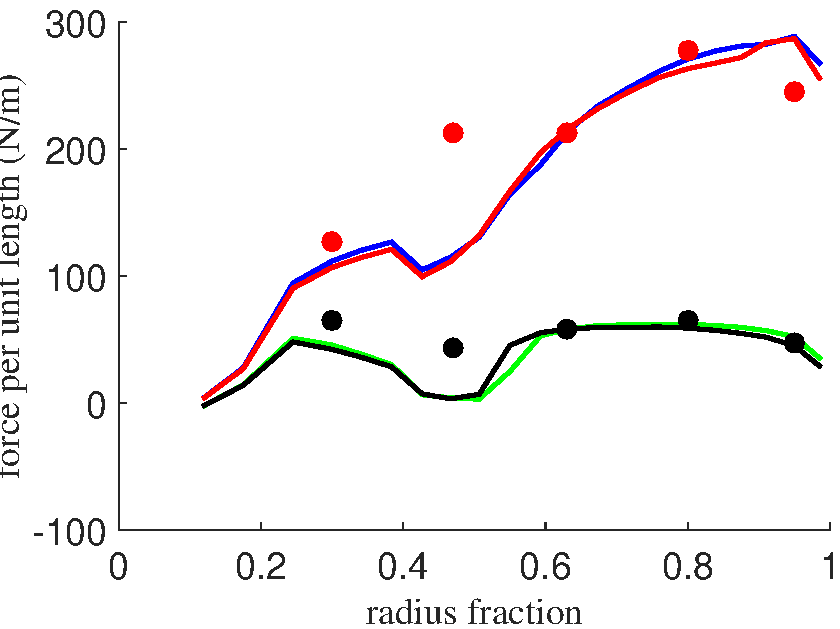
\includegraphics[width=0.3\textwidth]{images/Uinf_10}
   \label{fig:Uinf_10}
 }
 \caption{Distributed loads along blade at three different wind speeds with no yaw angle and a fixed azimuth ($\gamma = 0, \psi = 90^\circ$).  The circles corresponds to experimental data and the lines to simulation results.}
 \label{fig:Uinf}
\end{figure}


\Cref{fig:yaw_az90} and \cref{fig:yaw_az270} show the blade loading at six different yaw angles for two different azimuth angles (90 degrees azimuth in \cref{fig:yaw_az90}, and 270 degrees azimuth in \Cref{fig:yaw_az270}).  In each plot two different analysis methods are used.  The first method does not apply any corrections and is represented by the solid lines.  It does make use of the local velocity computation (\cref{eq:Vrel}), which is a function of yaw and azimuth.  The second method is the Pitt/Peters model (\cref{eq:pitt}) and is represented by a dashed line.  At yaw angles of 0 and 90 degrees, these two methods are identical.  We note that even with no correction (other than the local velocity calculation) the BEM model does reasonably well at predicting the load distribution across a wide range of yaw angles.  The Pitt/Peters model does capture the expected drop in loading on the downwind side (positive yaw, 90 degree azimuth), and conversely it captures the increase in loading for the upwind side at $270^\circ$ azimuth.  However, the magnitude of the correction appears to be too large, especially at large yaw angles.  At yaw angles larger than $30^\circ$ the Pitt/Peters model significantly underpredicts the loading along the blade (or overpredicts at 270 degrees azimuth).  For modest yaw angles, under $30^\circ$, the Pitt/Peters model may be beneficial.   

\begin{figure}[htbp]
\centering
 \subfloat[$\gamma = 0^\circ$]{
   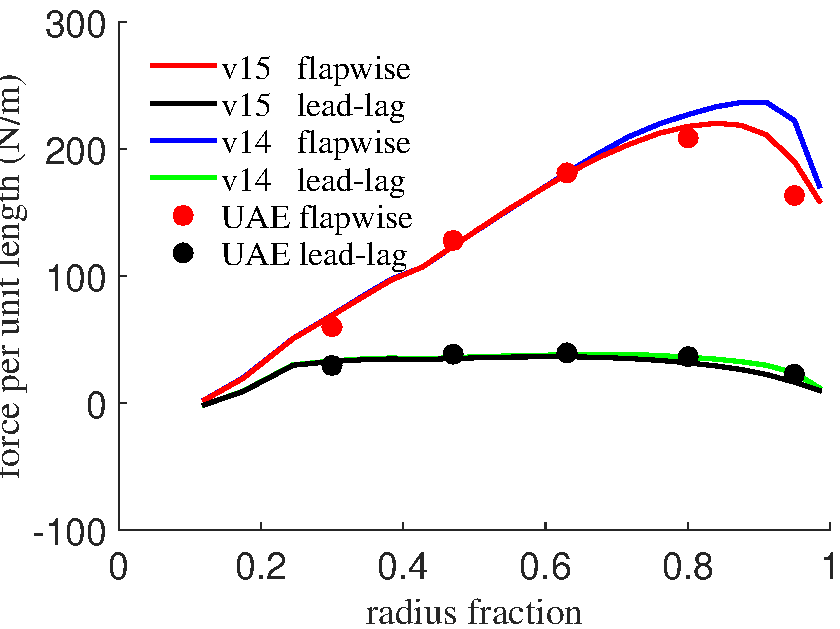
\includegraphics[width=0.3\textwidth]{images/yaw_0_az_90}
   \label{fig:yaw_0_az_90}
 }
 \quad
 \subfloat[$\gamma = 20^\circ$]{
   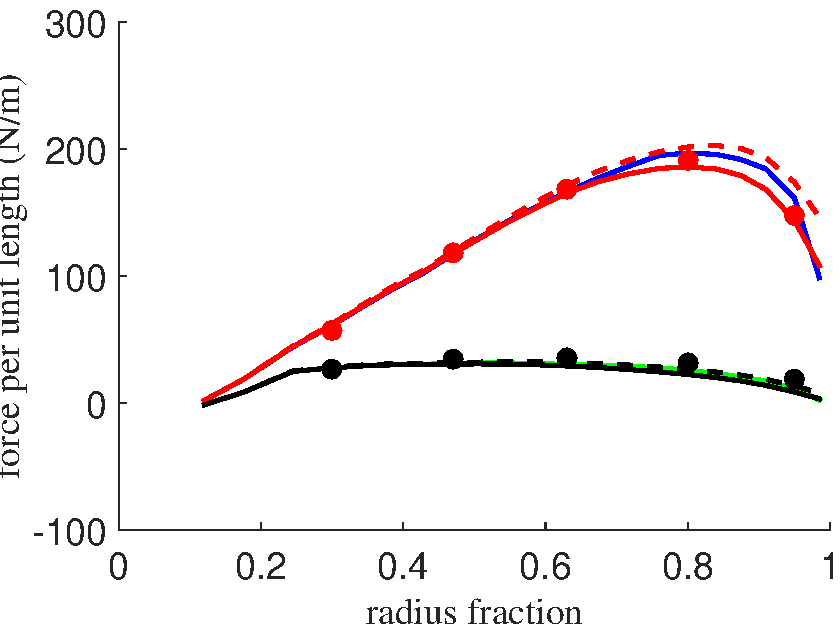
\includegraphics[width=0.3\textwidth]{images/yaw_20_az_90}
   \label{fig:yaw_20_az_90}
 }
 \quad
 \subfloat[$\gamma = 40^\circ$]{
   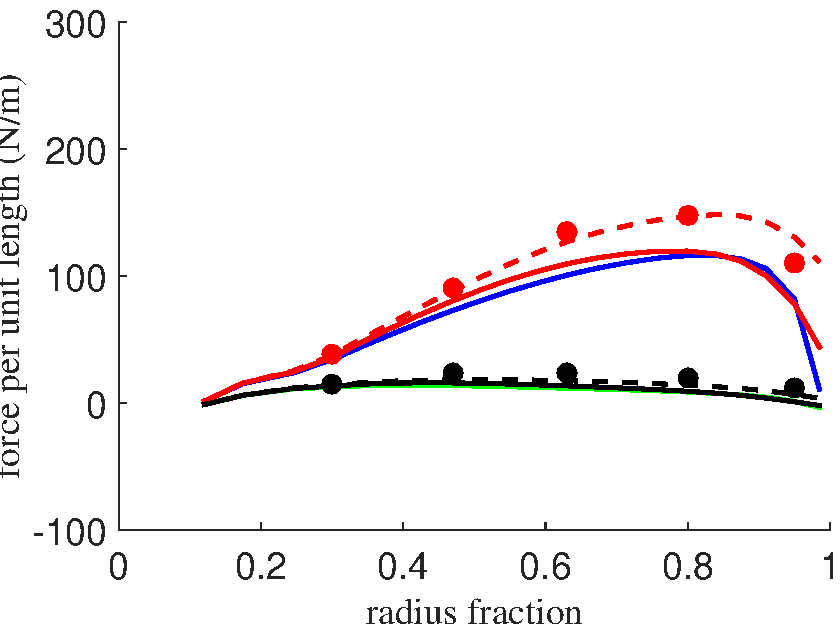
\includegraphics[width=0.3\textwidth]{images/yaw_40_az_90}
   \label{fig:yaw_40_az_90}
 }\\
 \subfloat[$\gamma = 60^\circ$]{
   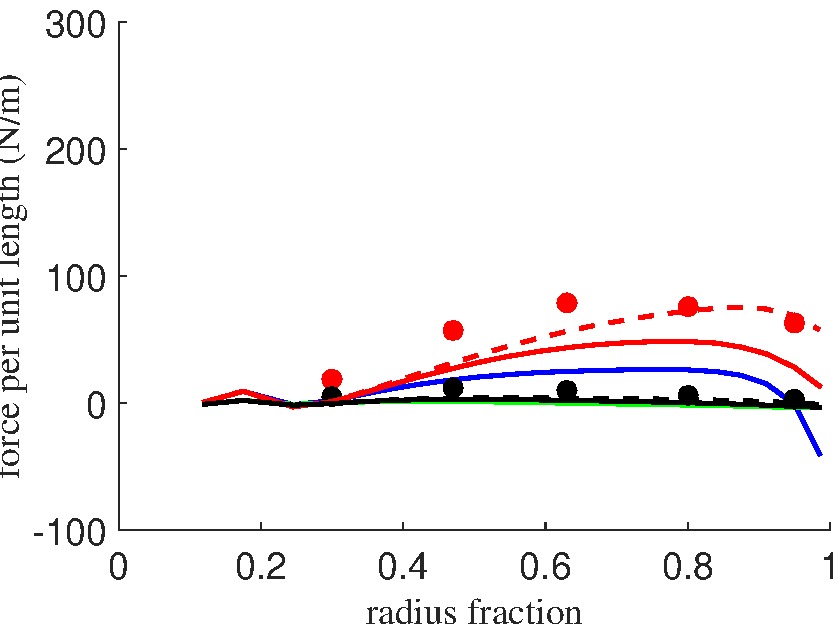
\includegraphics[width=0.3\textwidth]{images/yaw_60_az_90}
   \label{fig:yaw_60_az_90}
 }
 \quad
 \subfloat[$\gamma = 75^\circ$]{
   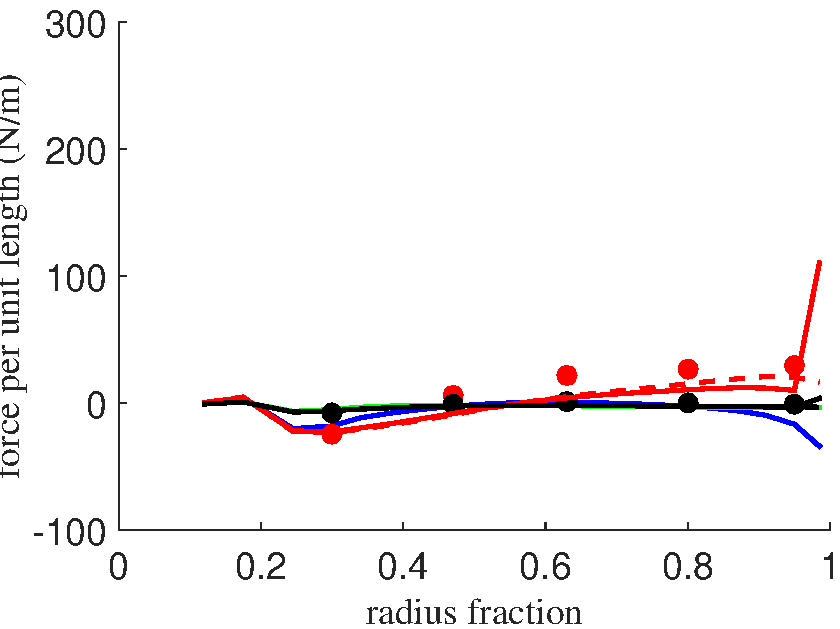
\includegraphics[width=0.3\textwidth]{images/yaw_75_az_90}
   \label{fig:yaw_75_az_90}
 }
 \quad
 \subfloat[$\gamma = 90^\circ$]{
   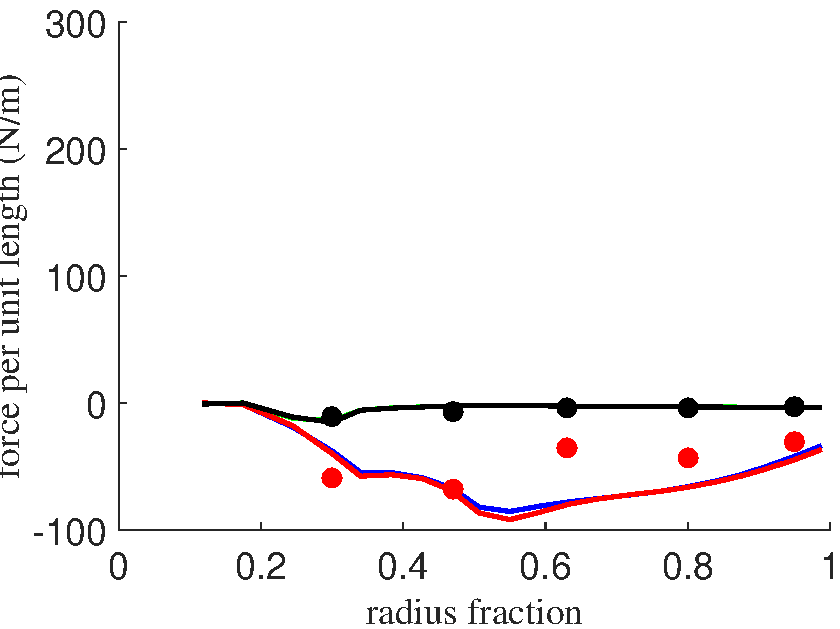
\includegraphics[width=0.3\textwidth]{images/yaw_90_az_90}
   \label{fig:yaw_90_az_90}
 }
 \caption{Distributed loads along blade at six different yaw angles ($V_\infty = 7 \textrm{ m/s}, \psi = 90^\circ$).  The closed circles represent experimental data, the solid lines are unmodified BEM results, and the dashed lines include the Pitt/Peters correction.}
 \label{fig:yaw_az90}
\end{figure}


\begin{figure}[htbp]
\centering
 \subfloat[$\gamma = 0^\circ$]{
   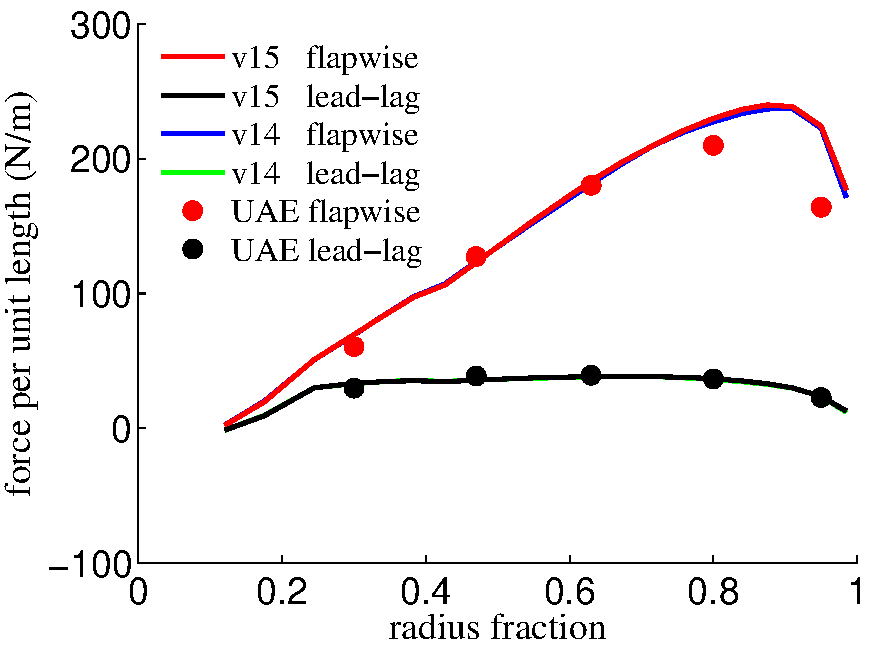
\includegraphics[width=0.3\textwidth]{images/yaw_0_az_270}
   \label{fig:yaw_0_az_270}
 }
 \quad
 \subfloat[$\gamma = 20^\circ$]{
   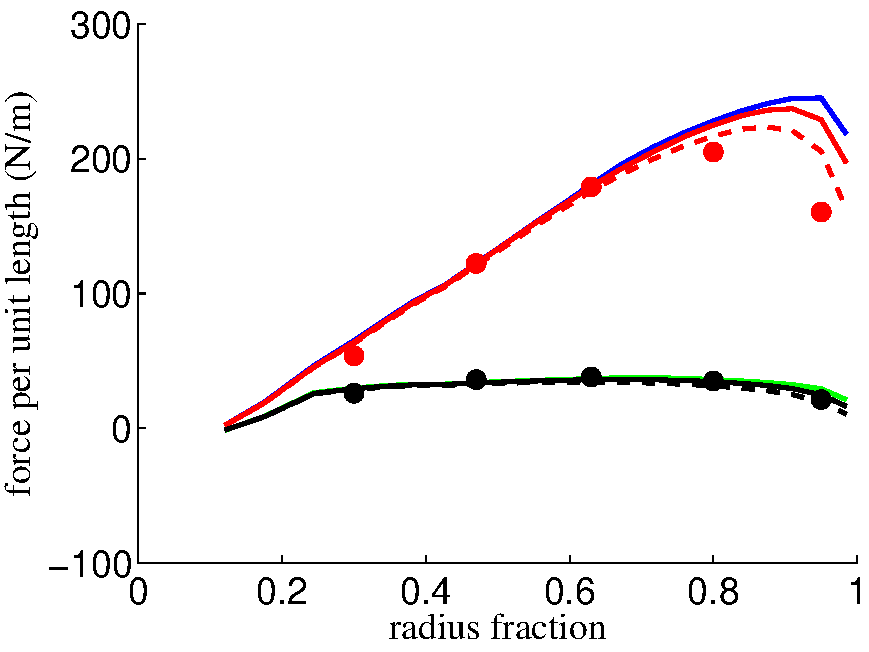
\includegraphics[width=0.3\textwidth]{images/yaw_20_az_270}
   \label{fig:yaw_20_az_270}
 }
 \quad
 \subfloat[$\gamma = 40^\circ$]{
   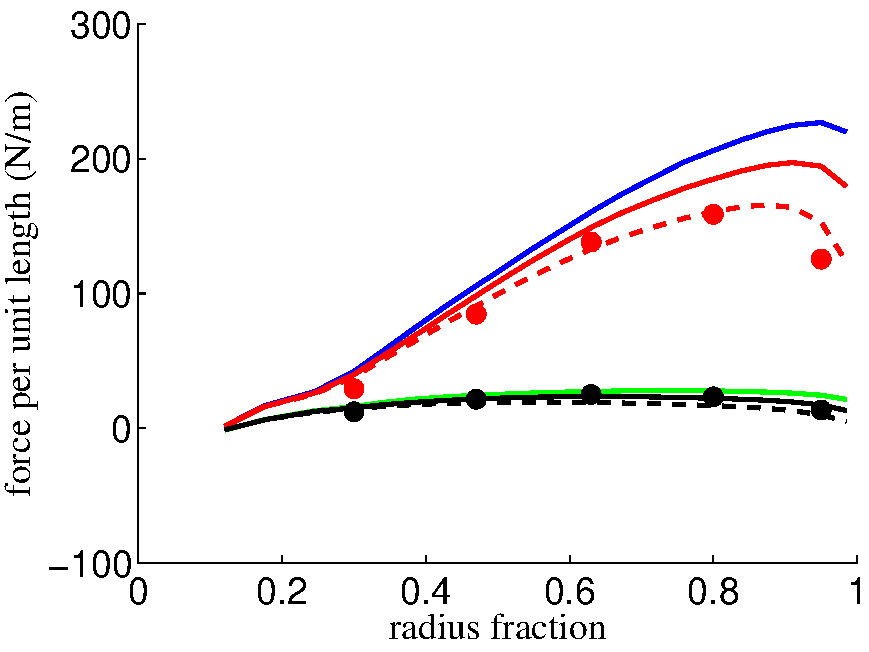
\includegraphics[width=0.3\textwidth]{images/yaw_40_az_270}
   \label{fig:yaw_40_az_270}
 }\\
 \subfloat[$\gamma = 60^\circ$]{
   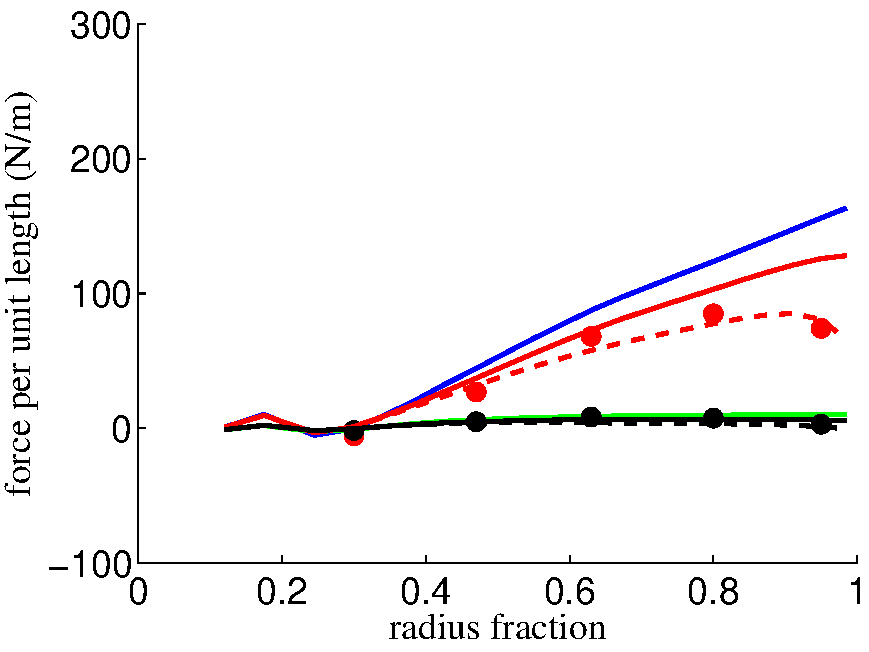
\includegraphics[width=0.3\textwidth]{images/yaw_60_az_270}
   \label{fig:yaw_60_az_270}
 }
 \quad
 \subfloat[$\gamma = 75^\circ$]{
   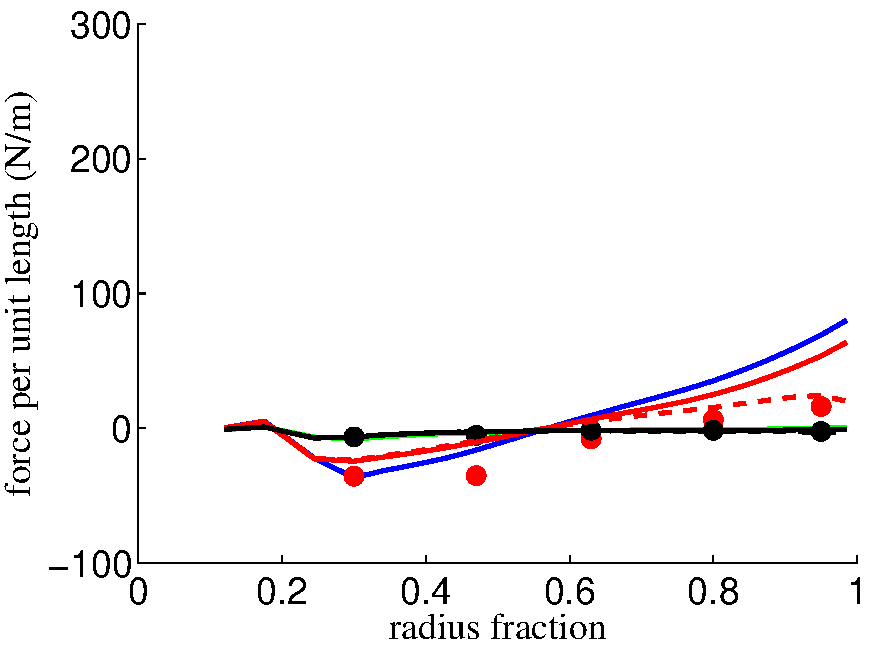
\includegraphics[width=0.3\textwidth]{images/yaw_75_az_270}
   \label{fig:yaw_75_az_270}
 }
 \quad
 \subfloat[$\gamma = 90^\circ$]{
   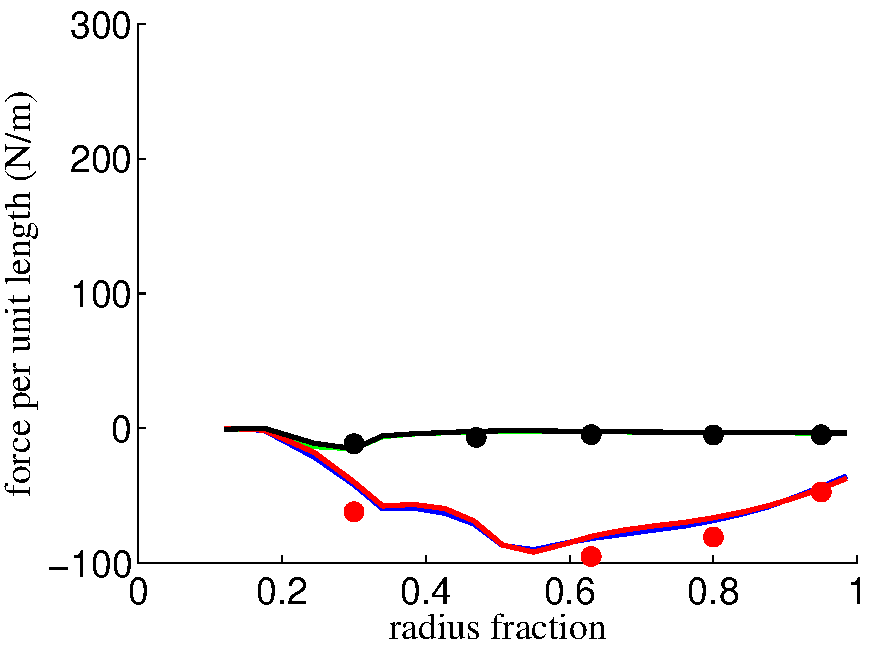
\includegraphics[width=0.3\textwidth]{images/yaw_90_az_270}
   \label{fig:yaw_90_az_270}
 }
 \caption{Distributed loads along blade at six different yaw angles ($V_\infty = 7 \textrm{ m/s}, \psi = 270^\circ$).  The closed circles represent experimental data, the solid lines are unmodified BEM results, and the dashed lines include the Pitt/Peters correction.}
 \label{fig:yaw_az270}
\end{figure}


\Cref{fig:azimuth_Np,fig:azimuth_Tp} show the variation in flapwise and lead-lag loads as a function of azimuth angle at three different radial stations along the blade.  Each plot is done at a fixed wind speed of 7 m/s and a fixed yaw angle of 20$^\circ$.  We see that the Pitt/Peters model does a better job at capturing the shape of the variation because it is able to capture the asymmetry.  However, the Pitt/Peters correction often overpredicts the amplitude of the variation, particularly towards the blade tips.  

\begin{figure}[htbp]
\centering
 \subfloat[$r/R = 0.3$]{
   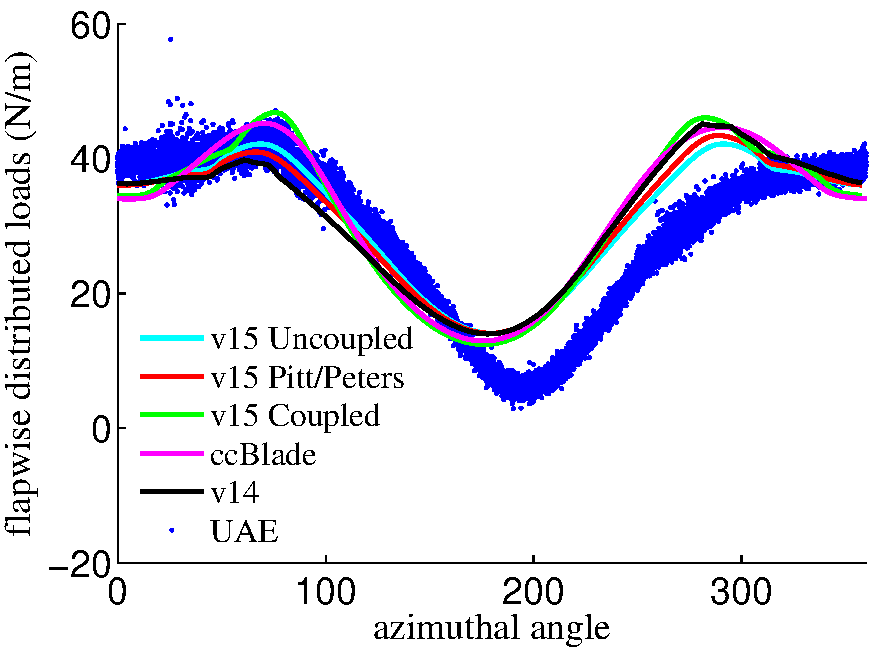
\includegraphics[width=0.3\textwidth]{images/station_Np_30}
   \label{fig:station_Np_30}
 }
 \quad
 \subfloat[$r/R = 0.63$]{
   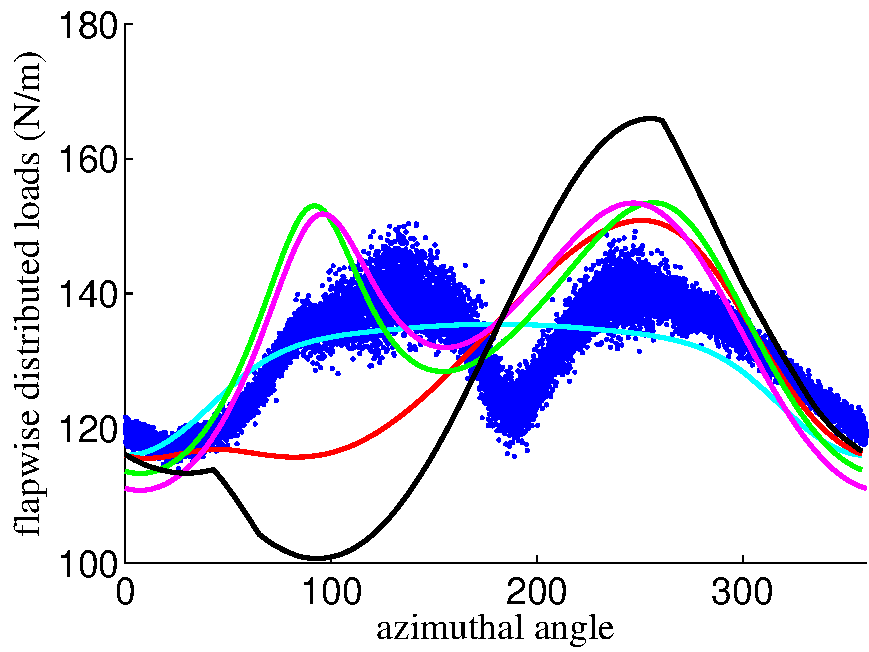
\includegraphics[width=0.3\textwidth]{images/station_Np_63}
   \label{fig:station_Np_63}
 }
 \quad
 \subfloat[$r/R = 0.95$]{
   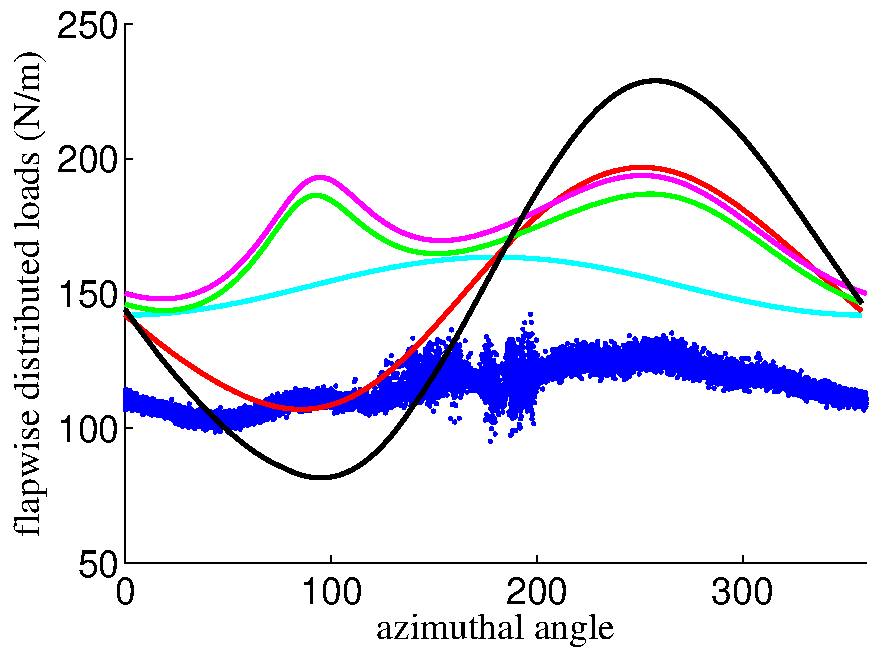
\includegraphics[width=0.3\textwidth]{images/station_Np_95}
   \label{fig:station_Np_95}
 }
 \caption{Flapwise loads at different stations along the blade as a function of azimuth ($V_\infty = 7 \textrm{ m/s}, \gamma = 20^\circ$). The circles are from the experimental data, the solid line from standard BEM theory, and the dashed line with the Pitt/Peters correction.}
 \label{fig:azimuth_Np}
\end{figure}


\begin{figure}[htbp]
\centering
 \subfloat[$r/R = 0.3$]{
   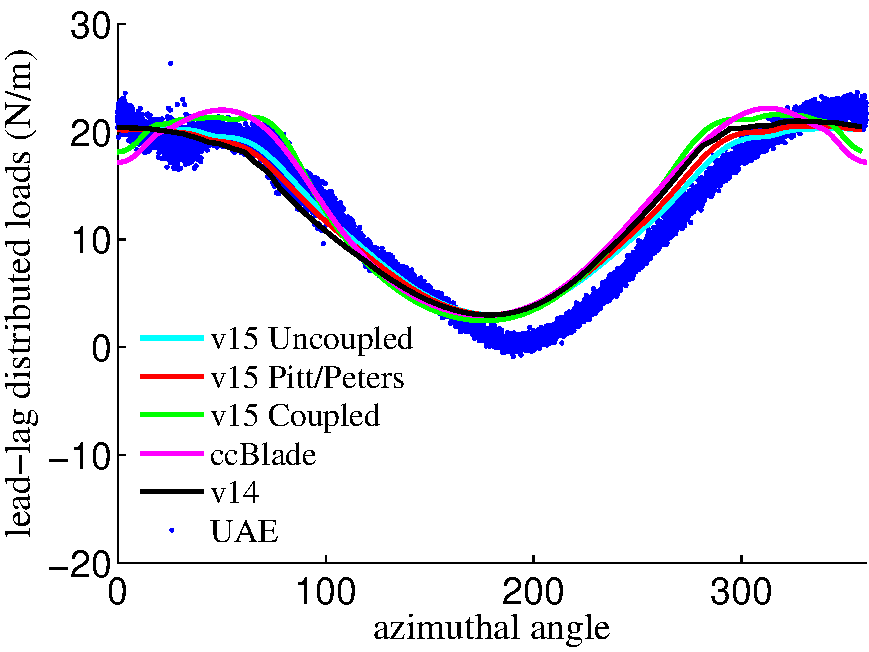
\includegraphics[width=0.3\textwidth]{images/station_Tp_30}
   \label{fig:station_Tp_30}
 }
 \quad
 \subfloat[$r/R = 0.63$]{
   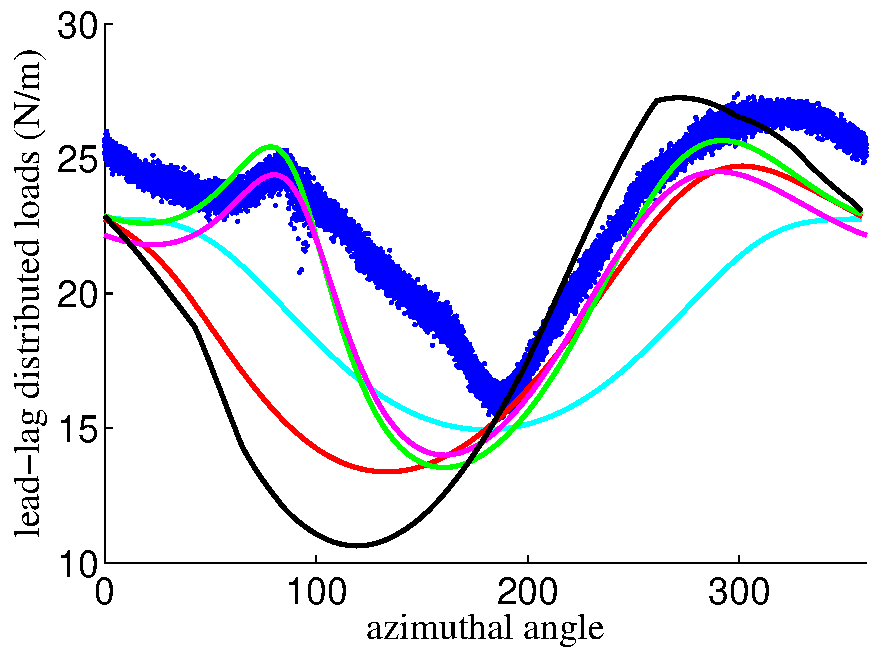
\includegraphics[width=0.3\textwidth]{images/station_Tp_63}
   \label{fig:station_Tp_63}
 }
 \quad
 \subfloat[$r/R = 0.95$]{
   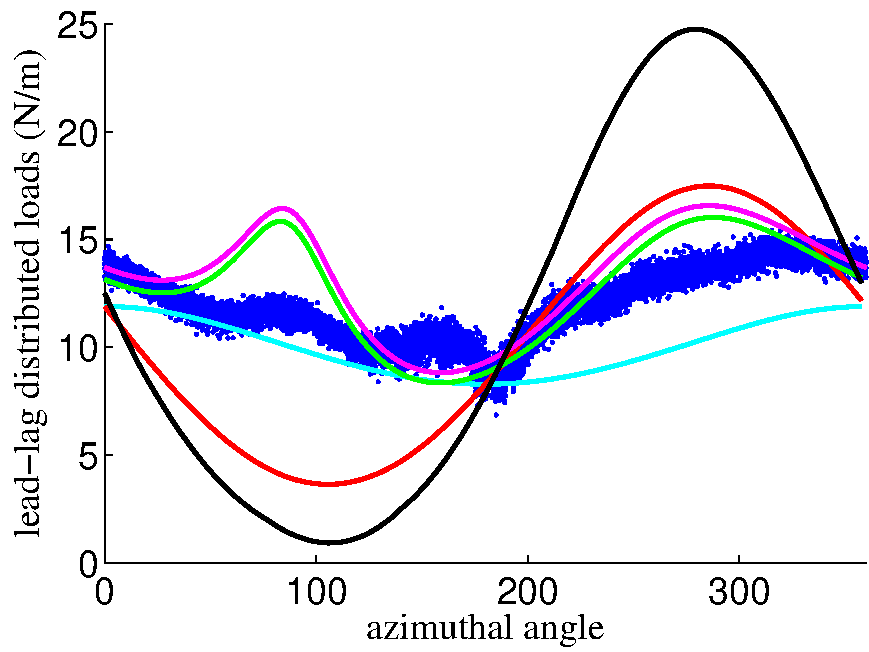
\includegraphics[width=0.3\textwidth]{images/station_Tp_95}
   \label{fig:station_Tp_95}
 }
 \caption{Lead-lag loads at different stations along the blade as a function of azimuth ($V_\infty = 7 \textrm{ m/s}, \gamma = 20^\circ$). The circles are from the experimental data, the solid line from standard BEM theory, and the dashed line with the Pitt/Peters correction.}
 \label{fig:azimuth_Tp}
\end{figure}

\FloatBarrier
\subsection{Coupled Methods}
[TODO]

\section{Conclusion}

This paper has discussed updates to AeroDyn, in particular improvements in the BEM solution algorithm and the skewed-wake modeling.  Comparisons have been shown between the old approach in Aerodyn, the new approach in AeroDyn using different approaches, and experimental data.  We have seen that just accounting for the velocity changes along the blade as a function of yaw, gives reasonably accurate results across a wide range of yaw angles.  The inclusion of the Pitt/Peters corrections improves the shape of the variation across azimuth angles, but does not necessarily lead to more accurate loading along the blades.  Current efforts are underway to include the coupled solution methodology, to explore other skewed wake models, add unsteady aerodynamic models, include a generalized dynamic wake option, and to couple the aerodynamics with the structural analysis in FAST v8.

\section*{Acknowledgments}
This work was supported by the U.S. Department of Energy under Contract No. DE-AC36-08GO28308 with the National Renewable Energy Laboratory.


\bibliographystyle{aiaa}
% \bibliography{/Users/andrewning/Dropbox/BYU/Papers/wind}
\bibliography{wind}


\end{document}
